%-*- coding: UTF-8 -*-
\documentclass[forprint]{WHUMaster}
% 选项 forprint: 交付打印时, 建议加上此选项, 以消除彩色链接文字, 避免彩色字迹打印偏淡.
% 选项为空:链接会彩色,会有多余空白页
% 选项 forlib: 提交给图书馆的电子版, 需要加上选项forlib,
%以消除空白页和彩色链接.

%%%=== 图片路径=== %%%
\graphicspath{ {figures/} }        % 图片放在 figures 文件夹.
%------------------------------
%\bibliographystyle{whuthesis} % 宏包natbib参考文献样式
\bibliographystyle{humannat} % 宏包natbib参考文献样式
%=====================================================
\begin{document}
%----------------------------------------------------
\fenleihao{}  % 根据自己学科填写!!!
\miji{}
\UDC{}
\bianhao{10486}
%------------------标题信息--------------------------
\title{波形拟合反演震源机制的定权研究及误差评定}
\Etitle{Weighting improvement and error estimation for inversion of mechanism from waveform}
\author{邓东平}
%\author{~}
\StudentNumber{2013202140004}
%\StudentNumber{~}
\Eauthor{Deng Dongping}
%\Eauthor{~}
\Csupervisor{朱良保\quad 教授}
%\Csupervisor{~}
\Esupervisor{Prof.~Zhu Liangbao}
%\Esupervisor{~}
\Cmajor{固体地球物理学}       %专业名
\Emajor{Solid Geophysics}
\Cspeciality{地震学}          %研究方向
\Especiality{Seismology}
%\Schoolname{School of Geodesy and Geomatics}
\Schoolname{~}
\date{二〇一六年四月}
\Edate{April, 2016}
%------------------------------------------------------
\pdfbookmark[0]{封面}{title}         % 封面页加到 pdf 书签
\maketitle   %生成中文封面
%---------------------------------------
% !Mode:: "TeX:UTF-8"

%%% 此部分包含: (1) 英文封面 (无需改动) ; (2) 郑重声明 (无需改动).

%%%%%%%%%%%%%%%%%%%%%%%%%%%%%
%%% -------------  英文封面 (无需改动)-------------   %%%
%%%%%%%%%%%%%%%%%%%%%%%%%%%%%
\thispagestyle{empty}
\renewcommand{\baselinestretch}{1.5}  %下文的行距
\vspace*{0.5cm}

\begin{center}{\zihao{2} \the\Etitle \par}\end{center}

\vfill

\begin{center}
\zihao{4}
\begin{tabular}{ r l }
 Candidate:      &  {\sc \the\Eauthor}      \\
 Student Number: & {\the\StudentNumber} \\
 Supervisor:     &  {\sc \the\Esupervisor}   \\
 Major:          & \the\Emajor  \\
 Speciality:     & \the\Especiality
\end{tabular}

\vspace*{2cm}
\begin{center}
  \iflib % 向图书馆提交电子文档, 使用黑白校徽.
  
\includegraphics[height=4cm]{whu.eps}       %%  黑白的. 很小, 只有 10k.
  \else
     \ifprint % 文档打印, 使用黑白校徽.
  
\includegraphics[height=4cm]{whu.eps}       %%  黑白的.
  \else
  
\includegraphics[height=4cm]{whulogo.eps} %%  彩色的.
  \fi
  \fi
\end{center}


\zihao{-2}
\the\Schoolname\\
{\sc Wuhan University}

\vspace*{1.0cm}

\the\Edate

\end{center}
%%%%%%%--判断是否需要空白页-----------------------------
  \iflib
  \else
  \newpage
  \thispagestyle{empty}
  \cleardoublepage
  \fi
%%%%%%%-------------------------------------------------
%%%--- 加入``郑重声明'' --- %%%%%%%%%%%%%%%%%
{\pagestyle{empty}
\newpage
\vspace*{20pt}
\begin{center}{\ziju{0.8}\zihao{-2}\heiti 郑重声明}\end{center}
\par\vspace*{30pt}
\renewcommand{\baselinestretch}{2}
{\zihao{4} \songti %

本人的学位论文是在导师指导下独立撰写并完成的,
学位论文没有剽窃、抄袭、造假等违反学术道德、学术规范和侵权行为,
否则, 本人愿意承担由此而产生的法律责任和法律后果,
特此郑重声明.

\vskip2cm

\hspace*{4cm}学位论文作者(签名): \hspace{4cm} \hfill \\[1cm]
\hspace*{10cm}年 \hfill  月 \hfill 日\hspace{1cm}\hfill\par}

%%%%%%%--判断是否需要空白页-----------------------------
  \iflib
  \else
  \newpage
  \cleardoublepage
  \fi
%%%%%%%-------------------------------------------------
}
\renewcommand{\baselinestretch}{1.6}
\small\normalsize 




 % 英文封面和郑重声明
%---------------------------------------
\frontmatter 
\pagenumbering{Roman}% 页码换成大写罗马数字
%--------------------------------------
% !Mode:: "TeX:UTF-8"

%%% 说明: 此部分需要自己填写的内容:  (1) 中文摘要及关键词 (2) 英文摘要及关键词

%%%%%%%%%%%%%%%%%%%%%%%
%%% ------------ 中文摘要 ---------------%%%
%%%%%%%%%%%%%%%%%%%%%%%
\begin{cnabstract}
近年来,利用波形拟合方法反演震源机制的方法已经越来越普遍,在震源研究中获得了广泛应用。由于震源机制反演问题具有解空间较小,反演公式复杂等特点,一个比较合适的反演算法是格点搜索反演。在实际应用波形拟合研究震源机制的工作中,也证实了格点搜索反演在该问题的适用性。格点搜索算法是指将解空间按一定精度划分为大量网格,并将一个网格范围内无数连续的解当成同一个解,因而实现了解空间的数值离散化。解算时依次遍历所有格点,试探性利用格点值求解相应观测量的理论值,并比较理论值与观测值匹配度,求最优解的过程便是寻求具有最高匹配度的格点值。

格点搜索算法仅需要计算待求模型到观测量的正演公式,因而有效避免了复杂的震源机制与波形的反算公式。在获得便利的同时,也伴随着一个很大缺陷——无法直接评价误差。正是由于格点搜索不需要求算观测数据到估计解的反推公式,因而也无法得到误差传播矩阵,导致不能在搜索到最优解的同时获得对解的误差评价。虽然误差评价的重要性不言而喻,但在实际工作中可以发现绝大部分震源机制的反演研究中均没有提及对震源机制的误差评估。为了获得一定的误差信息,本文基于概率统计原理提出了一种方法。该方法通过利用观测数据的噪声信息重新随机生成噪声,并利用生成的噪声模拟大量的“观测”数据,对大量模拟数据进行多次反演,便得到了误差范围内的解集。通过对该解集进行统计分析,不仅可以得到震源机制各参数的误差信息,还能得到参数间的相关性信息。为了检验方法的有效性,文中设计了相关实验考查其误差范围的准确性。多次实验均发现本文所提方法准确地估计了波形数据的随机噪声“传播”给震源机制的误差。

由于震源机制的重要性,日常研究中经常需要进行震源机制反演。为避免重复工作,一些研究者将基于自己反演方案和算法完成的反演程序进行公开,供其它人使用,于是便有了各种开源的反演程序。在这些开源程序中,CAP(Cut And Paste)和CPS(Computer Programs in Seismology)两个程序都是受到广泛应用,且较为成熟的利用格点搜索算法反演震源机制的程序。两个程序分别体现了其作者的在反演中的观点,在CAP程序的相关文献中,详细介绍了反演时所使用的加权基于不同波形间振幅大小差异的考虑,而从CPS的源码中发现其加权主要考虑到不同波形数据信噪比优劣的不同。由于二者的权重均通过震中距估计,经分析发现其权重数值大小相互冲突。为了解决该矛盾并吸收两种加权方案中的有益观点,本文提出了综合考虑信噪比和振幅调节两方面的联合加权方案。此外,通过实例分析发现震中距难以描述信噪比或振幅的真实情况,并因此提出了用各波形数据信息直接计算信噪比或振幅,以精化权重的数值。经检验,联合定权确实能在一定程度上优化反演结果。

本文第一章介绍了震源机制研究的背景,发展历程和现状。其中着重强调了当前利用波形拟合反演震源机制方法中常见的误差缺失问题,以及CAP和CPS中出现的加权差异和可优化性。之后简要介绍了本文的工作目标和实现方法。第二章对波形拟合反演震源机制的相关理论以及格点搜索算法进行了详尽地推导,并介绍了加权优化和误差评价的理论基础。第三章设计了一系列理论实验,通过实际计算来进一步证明本文所提观点的正确性。第四章则是以2013年芦山地震为例,展示了将本文所提方法进行真实应用的效果,并对反演结果进行了大量分析,表征了结果的可靠性。第五章是对全文工作和相关思想的总结,期望对之后的相关研究起到一点参考作用。

\end{cnabstract}
\vspace{1em}\par\vfill

%%%--------- 关键词 -------- %%%
\cnkeywords{波形反演, 震源机制, 格点搜索, 误差评价}

%%%%%%%%%%%%%%%%%%%%%%%


%%%%%%%%%%%%%%%%%%%%%%%
%%% ------------ 英文摘要 ---------------%%%
%%%%%%%%%%%%%%%%%%%%%%%

\begin{enabstract}
Recently, It's getting more and more common to inverse waveform for source mechanism. Grid search technique turn out to be a good fit for this inversion problem, as the possible source mechanisms are limited, besides to deduce the inversion equation seems quite different. This technique is approved to be effective on application to waveform inversion by experience in relative works. Grid search technique is a way to get the best solution from possible solutions: Firstly, we divide the solution space into grids with specified step-length for treating a unit grid as a single point, by which we have discretized the solution space. Secondly, It's time to iterate on every single grid to test how it fit to the problem based on a chosen evaluation standard(least squared criterion, etc.). Finally, after iteration, we certainly get a best solution among the solution space.

By application of grid search technique, we avoid the process of deducing equation to the form of solution; however, it comes with a inherent disadvantage that error estimation isn't provided directly any more. Due to this disadvantage, most of research about getting mechanism by inversion of waveform just ignore the error estimation, although it's so essential to estimate your solution from observed data; observed data always comes along with unpredictable noise. To fix this problem,we come up with a new method based on probability theory: Firstly, we modeling the noise and learn how to produce similar noises as many as we need. Secondly, by adding the new noises and observed data up, we synthesize the simulated data with possible noise. Thirdly, we inverse the synthesis dependantly to get a reasonable biased mechanism. Then repeat synthesis and inversion, we get enough mount of possible mechanisms. By analysis of this solution set, we definitely get the error estimation of mechanism. In the end, we run some tests to testify the validity of the new error estimation method provided by this thesis.

Source mechanism is a basic model for other research; so researchers need to get them from time to time. To avoid repeating work, some brilliant programs are provided by their owner so that anyone can use them freely and focus more on their research. CAP(Cut And Paste) and CPS(Computer Programs in Seismology) turn out to be two very popular programs Among all the open source software for getting mechanism. They both use grid search technique to fulfill the task, while they are some difference in weighting. CAP cares about the influence from amplitude difference in waveforms; CPS focus on the other side that data with better Signal-to-Noise Ratio should have priority. Furthermore, as CAP and CPS both calculate weighting by source-station distance, the outcome of relative weighting seems contradiction from the two programs. By analysis, we realize the two different weighting method are both reasonable. To fix the contradiction and take advantage of each, we manage to unite them in a way. Besides, we find the evaluation from source-station distance is rough and we refine it by estimating it from the very waveform itself instead of distance. In the end, we certify the improvement of united weighting by some experiments.

In the first chapter we introduce the background of source mechanism, the history of researching mechanism and current state,especially the lack of error estimation and the possibility to improve weighting by combination of CAP and CPS. Then the purpose and main work is mentioned briefly. In chapter two, we present the deduction theorem of getting mechanism by inversing waveform, grid search technique and the method developed in this thesis to estimate error and improve weighting. In the third chapter, a series of experiments are designed to test the new method. Then in the forth chapter, we formally apply the whole theory to a real earthquake, which happened in 20th April, 2013, in Lushan county. After inversion, a discussion is given to verify the result. Finally, in the last chapter, we give a conclusion of all work and some experience, and hope it helps when some others are doing the similar research.

\end{enabstract}
\vspace{1em}\par\vfill

%%%------ 英文关键词 ------- %%%
\enkeywords{waveform inversion, source mechanism, grid search technique, error estimation}
 %中英文摘要
%-------------------------------------
%---把目录加入到书签---%%%%%%%%%%%%%%
\pdfbookmark[0]{目录}{toc}%%%%%%%%%%%%
\tableofcontents
%---------------------------------------
\mainmatter % 开始正文
\baselineskip=20pt %正文行距20磅
%---------------------------------------
\chapter{引言}

\section{研究意义}

众所周知地震灾害是关系到国计民生的重大自然灾害,虽然极具破坏的大地震发生频率很低,但是一次地震所爆发的能量却是与吨级核爆相当\citep{Stein2003},其破坏性不言而喻。如2008年5月12号的汶川地震是自唐山地震以来在我国发生的导致直接死亡人数最多,经济损失最大的重大地震,其影响震惊海内外。然而,另一方面,地震的高能量所激发的高穿透力的地震波却是地震学家研究地球结构的福音,是人类目前研究地球内部结构的最有力工具。所以,无论从人民生活安全,经济保障,还是从科学探索的角度看,地震学研究都是很有意义的。

地震学研究的主要内容包括震源以及地下结构研究,震源机制是震源最基本的参数之一,其结果可进一步应用于理论震动图计算\citep{Wald2005}、海啸模拟\citep{Satake2007}、库仑应力转移估计\citep{King2007}、区域的应力分析和震源破裂过程反演中\citep{Kilb2001}。此外,利用已知震源机制计算得到面波震动图,用于在介质结构研究中代替到时或面波频散数据,以获得更多约束信息,直接拟合实际波形反演地下结构的方法也得到了广泛应用\citep{Nolet1990,Manaman2011,Friederich2003,Zielhuis1994,Cao2001,Lee1997}。因而在地震发生后,获得可靠的震源机制是有益且必要的。

由于真实情况下,获得的观测数据质量都不是完美的,为了得到更为准确和可靠的震源机制,需要在反演过程中尽可能优化结果。理论上,在给定观测数据和目标函数情况下,对于结果的最直接调控来自于反演的权重。合理的权重能使得对现有数据中有用信息更充分的应用,并压制无效噪声对反演的干扰影响。不同的加权得到的结果往往有差异,为了反演得到更“真实”的震源机制,必须谨慎考虑,合理地为数据加权。

另一方面,因为数据中的噪声具有随机性,使得反演结果相对真值有不可准确预料的偏差。事实上,反演结果与真实值的偏差还来源于所需参考模型的误差,数值计算舍入误差,理论的近似引起的偏差等等系统性误差。在此仅关注研究数据噪声引起的误差,为了方便,本文之后所提的误差除非特别指出,否则均指数据随机噪声导致的震源机制误差。由于由噪声导致的误差不可精确预料,为了使结果具有科学参考价值,要求对可能的误差范围进行评估。排除数据噪声影响的“理想”结果则包含在反演结果的误差范围内,虽然无法直接求出该“理想”结果,但至少能在一定置信区间内给出可靠的结果范围,对于借鉴以及进一步深入研究均具有重要意义。此外,对于某些算法而言(如本文反演所用的格点搜索算法),无论结果是否可信反演后均会得到一个“最优解”,但当涉及病态反演问题时,该震源机制很可能与真实情况有非常大偏差,未经过误差评定,结果可能对之后研究者具有误导作用。

\section{研究发展历程}

\subsection{方法分类}

利用地震波信息反演震源机制根据反演数据源差异主要可以分为三大类方法。第一类是P波极性反演,利用了初至波第一次起跳方向信息约束震源,但对台站分布要求高,且结果不太稳定;第二类是用振幅定量信息反演,利用各震相振幅的差异或方位特性等定量信息进行反演,但续至波的振幅测量通常比较困难;第三类是波形拟合反演,直接利用整个波形数据的所有可用信息计算震源机制,约束效果相对更好。

\subsection{P波初动极性反演}

震源机制反演研究早期,主要根据P波辐射花样在四象限的分布规律,利用初动极性符号对震源进行约束\citep{Balakina1961}。这种方法首先起源于\citet{Reid1910}在1906年旧金山地震研究\citep{Milne1910}基础上提出了弹性回跳理论——认为地震是由于地壳中岩石积累了过多应变能,超过其承受能力后,发生弹性断裂,势能随之释放。之后,人们发现了P波初动符号的分布规律\citep{Nakano1923},并提出了地震节面的概念。并开始利用地震台站记录到的地震波初动极性信息在被地震节面分隔的四象限空间的分布,对震源节面进行约束,进而得到震源机制。然而由于该方法仅使用了P波初动极性这一少量信息,并且初动极性的明显性与初动P波振幅相关。理论上P波初动极性及振幅大小所形成的辐射花样在节面分隔的四象限中分布如\reffig{fig1_01},可以发现,在节面上P波理论振幅为零。因此在节面附近,振幅微弱的P波信号可能受噪声影响,难以识别正确的初动符号。以上原因导致该方法适用性受限,且结果不太稳定,为了得到稳定结果该方法对台站的数量和分布要求很苛刻。
\begin{figure}
\centering
  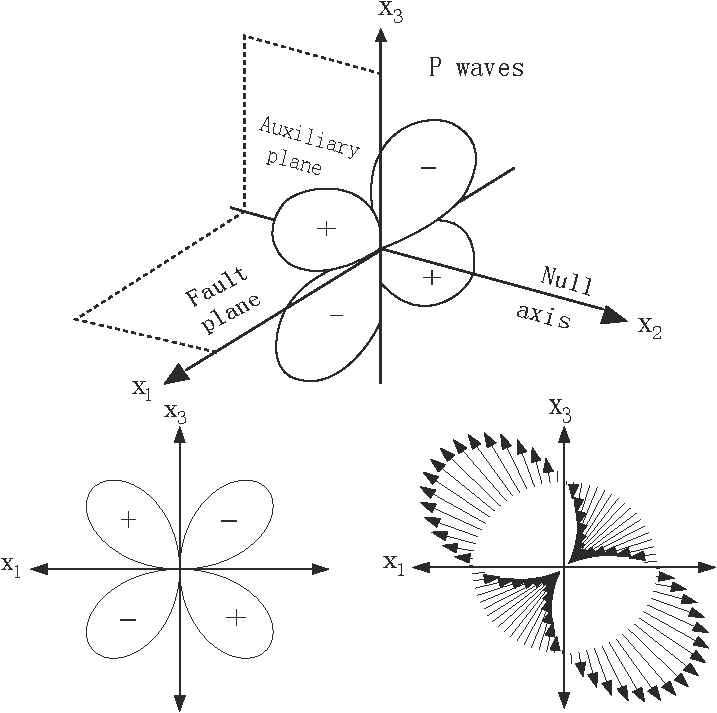
\includegraphics[scale=0.8]{fig1_01.pdf} 
  \caption{断层面($x_1$)和辅助面($x_3$)所分隔的四象限中P波辐射花样\citep{Stein2003}}
  \label{fig1_01}
\end{figure}

\subsection{振幅比反演}

第二类方法是利用各震相的振幅信息,使用波形振幅的定量数值信息,相对P波初动极性反演方法增加了反演数据的可用约束信息。这类方法包括利用P,S波的振幅比信息,通过同一台站不同分量震相信息比值规律,可一定程度避免来自介质模型不准确的系统性误差影响。其中利用P震相与SV震相的震幅比\citep{Kisslinger1982,Kisslinger1980}是一种行之有效的方案,并为了最大程度削弱介质模型对反演的影响,选择了直达上行地球表面的Z分量波。此外,在Kisslinger的研究基础上,\citet{wudaming1989}发现当有较高质量SH波时,通过P震相与SH震相的振幅比值反演可能得到相比P,SV振幅比反演更可靠的震源机制。另外,也有利用面波的振幅花样\citep{Stein2003}反演震源机制等可行方案。虽然利用振幅信息有效增强了对震源的约束,但是仍然对台站分布有较高要求,而且对近震波形S波初至振幅的测量,尤其是SV波的测量显得较为困难\citep{qiyuping2013},稍有不慎便可能得到较大偏差。

\subsection{波形拟合反演}

波形拟合反演直接利用了整个波形数据的所有信息进行反演,随着理论地震波的研究取得巨大成功\citep{Haskell1964,Herrmann1979,Wang1980}。在给定介质模型和震源机制情况下可以比较精确地计算出理论波形,使得直接使用观测波形数据与理论数据匹配反演震源机制的想法得以实现。通常波形中的体波数据由于穿透深,受浅层不均匀地壳结构影响较小,但考虑到体波衰减快,通常利用远震体波反演较大地震的震源机制,这能够减小地下介质模型横向非均匀性影响。而面波对介质结构较敏感,则较常用于具有较为精确介质参考模型的区域地震震源研究,或结合震源机制研究其较为敏感的地下结构\citep{Nolet1990}。由于波形数据相比初动极性或振幅,包含了更多有效信息,使得对台站数量及分布的要求有所降低,且结果更稳定、可靠,于是波形拟合反演的方法得到了快速发展和应用\citep{Walter1993,Ritsema1993,Zhao1994,Nabvelek1995}。

用地震波形拟合反演震源机制时,由于待求参数少、解空间有限且观测方程直接求解比较复杂,所以该问题非常适合用非线性反演中的全局搜索算法。在实践中,得到广泛应用的CAP(Cut and Paste的简称)\citep{Zhao1994,Zhu1996,Tan2006}和CPS(Computer Programs in Seismology的简称)\citep{Herrmann1989}等波形拟合反演程序充分说明了全局搜索在震源机制反演问题中的有效性。

\section{研究现状及问题}

Herrmann开发的CPS软件包中用于震源机制反演的子程序和CAP均利用格点搜索方法反演震源机制,由于二者的实用性和开源性,被广泛应用于震源机制研究中。然而CAP和CPS加权方法的侧重点不同,前者考虑几何扩散导致波形振幅的衰减,给较低振幅的波形加大权重,以平衡不同振幅波形在反演中的影响力;后者则关注传播过程中信噪比的降低,赋予高信噪比数据较大权重。进一步考虑到波形振幅及信噪比与震中距间的关系,\citet{Zhu1996}在CAP中将权重设置为关于震中距递增的幂函数,而CPS方法中使用震中距的反比例函数作为权重值。幂函数和反比例函数的单调性恰巧相反,导致从数值上看,两种方法对同一套数据波形所定权重大小相互矛盾——CPS定权震中距较近台站权重较高,而CAP定权中则震中距较远台站相对权重较大。此外,通过实例计算及理论分析发现,实际观测波形的振幅及信噪比与震中距的关系较为复杂,难以用简单的初等函数进行描述,因此利用幂函数或反比例函数估算的振幅和信噪比均较粗糙。且由于函数中包含的某些辅助参数赋值因人而异,故无法准确体现数据的真实性和客观性。

另一方面,随着CAP、CPS等用波形非线性反演震源机制的算法得到广泛应用\citep{Luo2015,DAmico2014},其非线性反演中误差缺失的问题逐渐受到关注。考虑到误差评价的重要性,国内外学者均对震源机制反演的误差估计问题进行了研究,\citet{Duputel2012}从误差的来源入手,对震源机制进行误差评价,但其方法只适用于线性反演的震源机制误差估计。考虑到目前应用广泛的全局搜索反演,本文旨在探究能应用于非性线反演算法的误差评估方法。对于非线性反演,最常见的方法是对目标函数的极值人为给定一个阈值,满足该条件的所有解构成误差范围内解集,该方法简洁直观,能快速发现不同模型参数的误差相对大小关系,但是阈值的给定有主观性,导致定量结果难以让人信服。\citet{zhenjianchang2015}借鉴Bootstrap(Efron1979)的思想,对数据集随机多次选取子集进行独立反演并对解集样本用一定方法分析,以评估其整体误差及解。但是为使样本能反映整体,统计分析不仅要求样本抽取的随机性,还对原始样本大小有一定要求,当可用的地震记录数量不是很大时,可随机选择的子样本以及子样本总量难以满足统计要求,基于重抽样的该方法便不适用了。

\section{本文设定目标及方案}

针对以上分析,为了解决CPS和CAP反演定权方法出现的矛盾以及误差缺失问题,本文分别尝试进行权重优化以及误差评定。对于定权,结合CPS与CAP,综合考虑振幅衰减和信噪比差异影响,将二者统一计算权重,从而解决上述的权重数值矛盾问题。其次,计算时摈弃了用震中距简单函数估算振幅或信噪比方案,而是基于每道波形数据自身的信息,准确评估振幅和噪声。由于没有人工干预,在提高精确度的同时有效保证了客观性。

针对反演震源机制时欠缺误差估计的问题,本文借鉴了\citet{Hardebeck2002}对P波初动极性反演方法稳定性改进的思路——首先估计离源角等观测数据的误差大小,据此模拟随机误差,并将其加入原始数据生成多组模拟数据集,最终反演得到一系列误差范围内的解集。该方法不仅估计了误差,且使得反演结果更稳定\citep{Hardebeck2002}。将该思想应用到波形反演震源机制的问题中,通过评估噪声随机模拟多套波形数据集,并用每套数据分别独立进行反演,得到包含多个反演结果的解集,最后对解集统计分析得到解的误差。本文方法与\citet{zhenjianchang2015}的重采样类方法不同的是每次反演的数据并非原始数据集的子集,而是与数据集等价的模拟数据集,保留了原数据集的样本大小,更重要的是每套数据均具有一致的数据分布结构。对观测数据的数量要求相对降低,理论上能比重采样类方法更好应用于台站记录较稀少的地震事件。

为了验证本文提出权重优化方案和误差评价方法的有效性,基于CPS反演程序进行了一系列理论试验,分别检验权重优化效果和误差估计与理论预测是否吻合。对同一个设定条件下的模拟地震进行了三次试验,分别测试权重优化的效果,误差评定方法对噪声的反应情况,误差评价时重复反演次数的设定值。第一次试验分别设定了单独信噪比加权,单独振幅调节加权,信噪比和振幅调节联合定权三组对照组。三组反演组结果相差不大,但联合反演组的综合偏差更小,体现了联合定权的优越性。第二次试验测试结果误差对数据噪声的反应是否合理,以证明误差估计方法的有效性,对理论事件加噪时分别加了低、中、高及超高强度噪声,反演结果确实体现了误差由低到高的趋势,而且增长率符合理论预测。理论真值均在各次反演的误差范围内,表明了本文误差估计结果的真实性。第三次试验研究误差评价时反演的重复次数对最终结果的影响,用以为该方法在应用时选择合适的反演次数。试验分别尝试了重复10次,50次,100次和200次,结果发现该方法在次数达到50次-200次之间对反演次数不是特别敏感,结果基本一致且可信。为同时保证样本量充足并节省计算时间,选定100次为默认反演次数。

为了检验本文误差估计方法和权重优化的实应性,以2013年4月20日的芦山地震为例,分别采取单独振幅调节加权、单独信噪比加权以及振幅调节和信噪比调节联合加权的策略进行三次反演,并对三次反演的结果进行误差估计。通过对结果的合理可靠性及稳定性两方面进行综合讨论比较,以真实案例证实本文联合加权策略反演结果最优,最终振幅调节和信噪比调节联合加权对应的震源机制解为(走向$211\degree\pm5\degree$,倾角$41\degree\pm1\degree$,滑动角$94\degree\pm2\degree$),震源深度17km,与其它研究者的研究成果有很好的一致性,且与震源区的应力及地质构造情况均相互吻合。
 %第一章 引言
%---------------------------------------
\chapter{原理分析}

\section{震源基础概念}
1906年旧金山发生了一次在地震学上具有重大研究意义的地震,地震前后对圣安德烈亚斯断层的研究结果\citep{Milne1910}使人们普遍认为发生地震的原因是震源处的断层发生了滑移错动,巨大的势能转化为了热能及地震波等能量。这种错动可由位错理论进行解释,位错理论认为地震的发生是因为应力长期缓慢的大量积累,最终达到了断层锁定的极限,引发断层面(原有断层或地震新生断层)两侧发生突然的位错,导致了应力释放并形成地震。如果断层在地表有出露,则相应会在地表看到走向线分隔的两盘沿着滑动方向的相互错动,如\reffig{fig2_01}所示。
\begin{figure}
\centering
  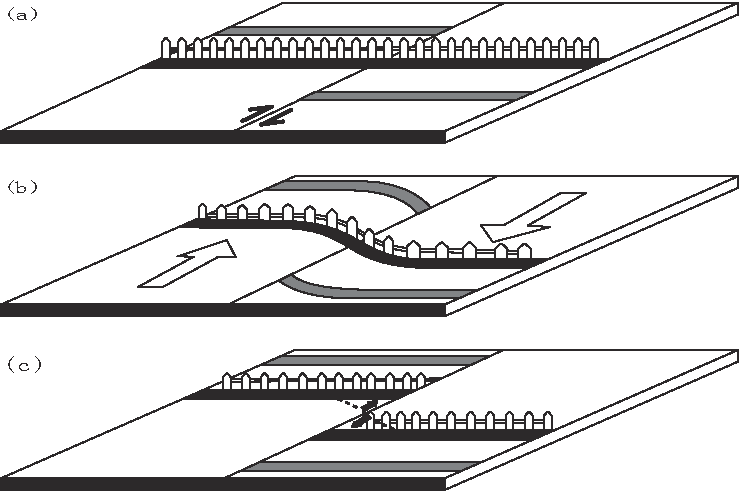
\includegraphics[scale=0.7]{fig2_01.pdf} 
  \caption{断层错动在地表的显现,(a)为震前,(b)为发震时,(c)为震后\citep{Stein2003}}
  \label{fig2_01}
\end{figure}

自此以后,对于地震震源的研究就开始集中到断层面的研究上。通常认为断层面两侧的应力在地震发生前后都是连续的,只有位移在断层面两侧突然间断,所以研究清楚断层面上的所有运动学信息是研究整个震源过程的主要内容。如果进一步简化,将地震发生时断层的位错视为纯剪切的点源位错(事实证明该简化很多情况下是合理的,且本文只讨论该情况),则利用三个描述断层的参数便可完整描述震源的物理过程(不考虑时间函数),并称该三参数为震源机制。求解震源机制的过程便是求解该三个参数的过程,该三参数具体定义如图\ref{fig2_02}所示。
\begin{figure}
\centering
  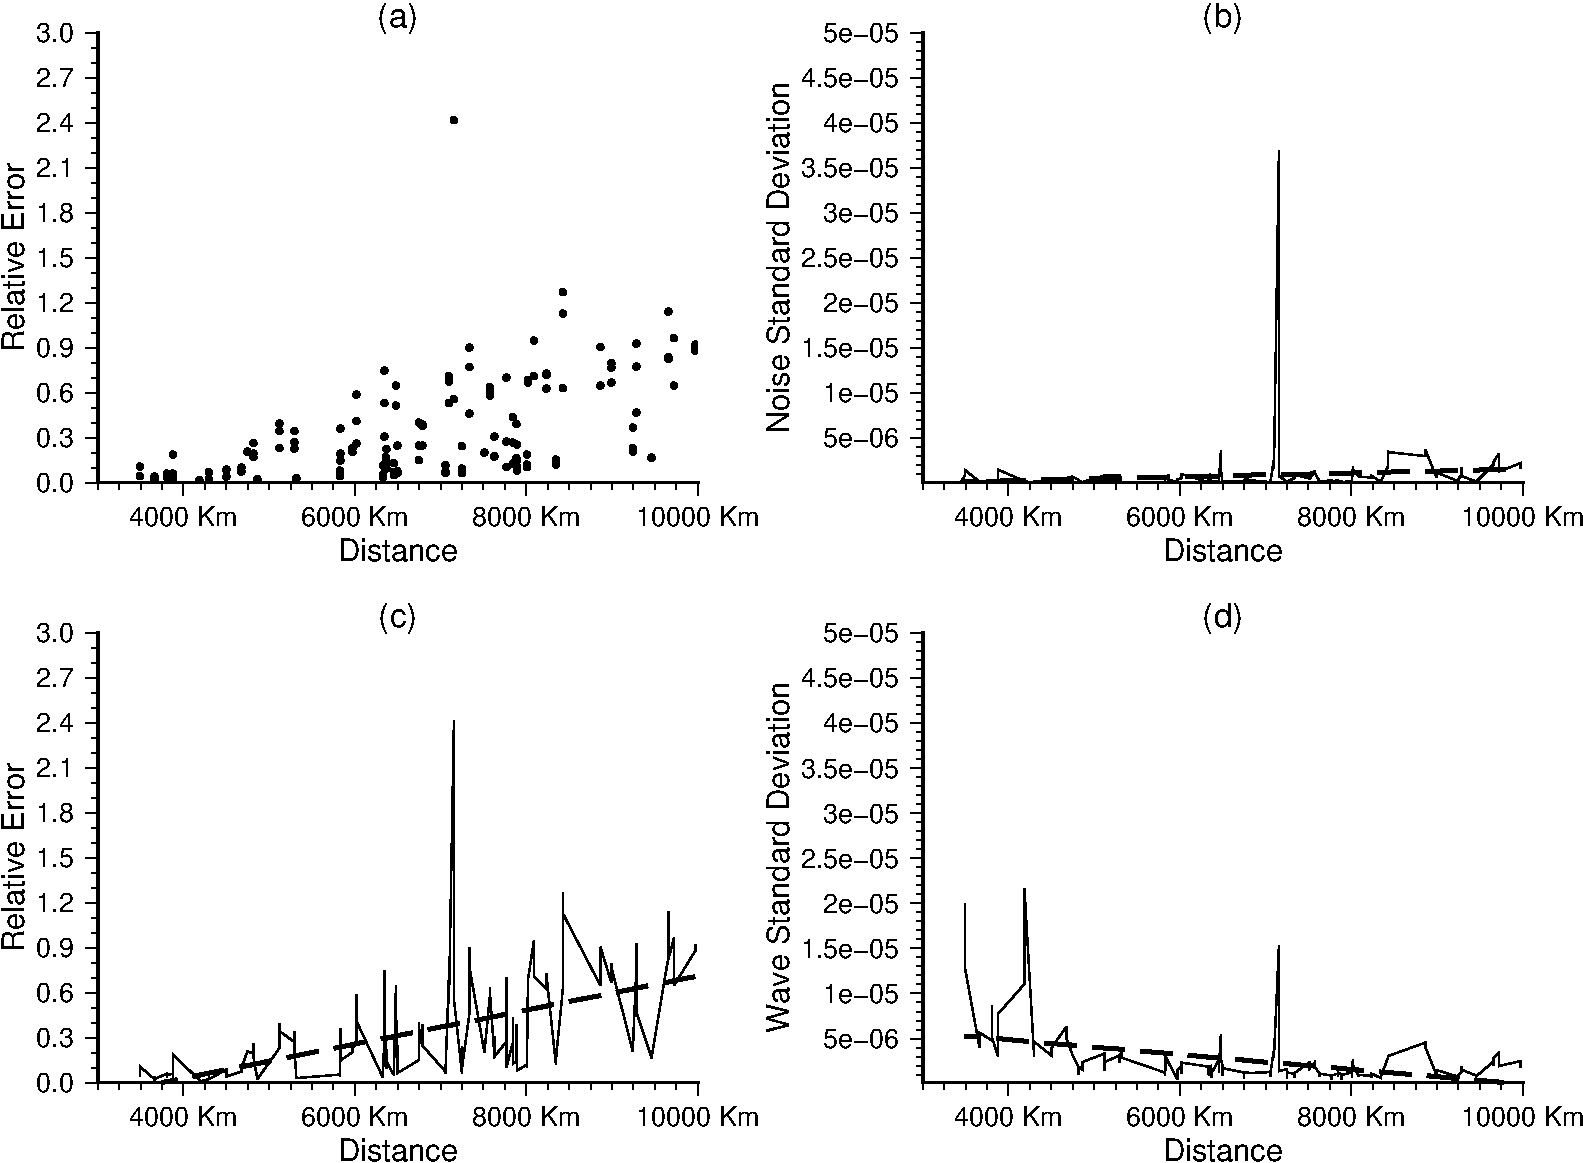
\includegraphics[scale=0.6]{fig2_02.pdf} 
  \caption{震源机制三个参数的具体意义,$\phi_s$、$\delta$、$\lambda$分别为走向、倾角和滑动角\citep{chengwanzheng2006}}
  \label{fig2_02}
\end{figure}

\section{波形拟合反演}

\subsection{波形分解}
理论研究表明,同步地震点源\citep{Silver1982}所激发的地震波场如\refeq{eq2_01}\citep{Jost1989}。
\begin{equation}
\label{eq2_01}
d_n(x,t)=M_{ki}[G_{nk,i}*s(t)]
\end{equation}

其中$s(t)$为震源时间函数,$M_{ki}$为地震矩张量,$G_{nk,i}$为格林函数,从上式可知理论波形$d_n$与地震矩张量$M_{ki}$为线性关系。根据\citet{Kikuchi1991}的分解方法,任意地震矩张量均可由6个简单地震矩张量通过线性组合而成,如\refeq{eq2_02}。
\begin{equation}
\label{eq2_02}
M=\sum_{k=1}^6a_kM_k
\end{equation}

\refeq{eq2_02}中等式右边的$M_k$如\refeq{eq2_03}所示。
\begin{equation}
\label{eq2_03}
\begin{array}{ccc}
M_1=\left[\begin{array}{ccc}
0 & 1 & 0\\
1 & 0 & 0\\
0 & 0 & 0\\
\end{array}\right]&
M_2=\left[\begin{array}{ccc}
1 & 0 & 0\\
0 & -1 & 0\\
0 & 0 & 0\\
\end{array}\right]&
M_3=\left[\begin{array}{ccc}
0 & 0 & 0\\
0 & 0 & 1\\
0 & 1 & 0\\
\end{array}\right]\\
M_4=\left[\begin{array}{ccc}
0 & 0 & 1\\
0 & 0 & 0\\
1 & 0 & 0\\
\end{array}\right]&
M_5=\left[\begin{array}{ccc}
-1 & 0 & 0\\
0 & 0 & 0\\
0 & 0 & 1\\
\end{array}\right]&
M_6=\left[\begin{array}{ccc}
1 & 0 & 0\\
0 & 1 & 0\\
0 & 0 & 1\\
\end{array}\right]\\
\end{array}
\end{equation}

$M_1$-$M_6$为6个简单的地震源,其中$M_6$代表爆炸源,其余5个均为剪切位错源,根据\refeq{eq2_02}和\refeq{eq2_03}推导可得到系数$a$与$M$各分量间的对应关系如\refeq{eq2_04}和\refeq{eq2_05}所示。
\begin{equation}
\label{eq2_04}
M=\left[\begin{array}{ccc}
a_2-a_5+a_6 & a_1 & a_4\\
a_1 & -a_2+a_6 & a_3\\
a_4 & a_3 & a_5+a_6\\
\end{array}\right]\\
\end{equation}

\begin{equation}
\label{eq2_05}
\left[\begin{array}{c}
a_1\\
a_2\\
a_3\\
a_4\\
a_5\\
a_6\\
\end{array}\right]=
\left[\begin{array}{c}
M_{12}\\
(M_{11}+M_{33}-2M_{22})/3\\
M_{23}\\
M_{13}\\
(2M_{33}-M_{11}-M_{22})/3\\
(M_{11}+M_{22}+M_{33})/3\\
\end{array}\right]
\end{equation}

将\refeq{eq2_02}代入\refeq{eq2_01},并省略波形分量指标$n$可得到\refeq{eq2_06}。
\begin{equation}
\label{eq2_06}
d=\sum_{k=1}^{6}a_kd_k
\end{equation}

再将\refeq{eq2_05}所示的$a$与$M$关系代入\refeq{eq2_06}可得到$d$关于$M$与$d_k$关系的\refeq{eq2_07}。
\begin{equation}
\label{eq2_07}
\begin{array}{rl}\\
d=&M_{11}(1/3d_2-1/3d_5+1/3d_6)+M_{12}d_1+M_{13}d_4\\
&+M_{22}(-2/3d_2-1/3d_5+1/3d_6)+M_{23}d_3\\
&+M_{33}(1/3d_2+2/3d_5+1/3d_6))
\end{array}
\end{equation}

为简化,将\refeq{eq2_07}中$M$矩阵的6个独立分量依次记为 $M_1,M_2,M_3,M_4,M_5,M_6$,并将与$Mi(i=1,2,..6)$相乘的关于$d_k$的多项式简记为$G_i(i=1,2,...6)$,于是得到了简洁的6项求和的理论波形\refeq{eq2_08}。在此我们按照\citet{Stein2003}专著中关于地震矩反演章节中对格林函数的推广定义,将\refeq{eq2_08}中的$G_i$也称为格林函数,此格林函数即是我们之后在CPS程序反演中需要用到的。
\begin{equation}
\label{eq2_08}
d=G_iM_i(i=1,2,...6)
\end{equation}

于是任意地震矩产生的波形均可由其矩张量矩阵和6个格林函数线性组合得到,而格林函数又可由6个已知基本地震矩激发的波形$d_k(k=1,2,...6)$叠加得到。由于以上运算均是线性运算,在$d_k$已知的情况下,在计算机中经几次迭加得到任意理论波形$d$速度非常快。

至此,我们已经将任意剪切位错源的波形分解为6个基本震源波形的线性叠加,而叠加的系数可由该位错源的震源机制唯一确定。现在的关键问题转化为计算6个基本震源对应的理论波形$d_k$,这可通过之后要介绍的格林函数库快速实现。

\subsection{格林函数库}

通常情况下天然地震由断层间错动造成,震源均近似纯剪切位错源。习惯上人们用破裂断层的三个角度参数——走向,倾角和滑动角来更直观地描述震源机制,对于纯剪切位错源,它们和地震矩张量是等价的,相互间的转换关系如\refeq{eq2_09}所示\citep{Aki1980}。
\begin{equation}
\label{eq2_09}
\left\{
    \begin{array}{l}
    M_{11}=-M_0(sin{\delta}cos{\lambda}sin{2\phi_s}+sin{2\delta}sin{\lambda}sin^2{\phi_s})\\
    M_{12}=M_0(sin{\delta}cos{\lambda}cos{2\phi_s}+1/2sin{2\delta}sin{\lambda}sin{2\phi_s})\\
    M_{13}=-M_0(cos{\delta}cos{\lambda}cos{\phi_s}+cos{2\delta}sin{\lambda}sin{\phi_s})\\
    M_{22}=M_0(sin{\delta}cos{\lambda}cos{2\phi_s}-sin{2\delta}sin{\lambda}cos^2{\phi_s})\\
    M_{23}=-M_0(cos{\delta}cos{\lambda}sin{\phi_s}-cos{2\delta}sin{\lambda}cos^2{\phi_s})\\
    M_{33}=M_0sin{2\delta}sin{\lambda}\\
    \end{array}
\right.
\end{equation}

其中,$\phi_s$是走向,$\delta$是倾角,$\lambda$是滑动角。 $M_0$是最早由\citet{Aki1966}提出的用来度量震源长周期辐射的强度,最初称为地震矩。由于是一个标量,现在又叫作标量地震矩,代表了地震的能量强度。将\refeq{eq2_09}代入\refeq{eq2_08}即可将公式进一步转化为理论波形关于震源机制三参数的形式。

现在我们研究6个基本地震对应的理论波形$d_k(k=1,2,..6)$如何计算,在均匀介质\citep{Ben-Menahem1963}和层状介质\citep{Haskell1964}模型的面波波场辐射理论基础上,\citet{Wang1980} 进一步研究了剪切位错源在层状速度模型中所激发的地震波场,其在柱坐标频域下如\refeq{eq2_10}所示。
\begin{equation}
\label{eq2_10}
\left\{
    \begin{array}{l}
    U_z(r,\phi,0,\omega)=Z_{SS}{\cdot}s_2+Z_{DS}{\cdot}s_3+Z_{DD}{\cdot}s_1\\
    U_r(r,\phi,0,\omega)=R_{SS}{\cdot}s_2+R_{DS}{\cdot}s_3+R_{DD}{\cdot}s_1\\
    U_{\phi}(r,\phi,0,\omega)=T_{SS}{\cdot}t_2+T_{DS}{\cdot}t_1\\
    \end{array}
\right.
\end{equation}

\refeq{eq2_10}中$s_1$, $s_2$等8个系数和震源相关,经推导\citep{mashutian1999}与震源机制三参数关系如\refeq{eq2_11}所示,\refeq{eq2_11}中$\phi$是地震观测台站相对震源的方位角,$\lambda$,$\delta$,${\phi}_s$分别代表断层滑动角,倾角,走向。\refeq{eq2_10}中的$Z_{SS}$,$R_{SS}$,$T_{SS}$分别对应于$\delta=90^\circ$,$\lambda=0^\circ$的纯走滑型断裂的理论地震图的垂向、径向、切向分量;$Z_{DS}$,$R_{DS}$,$T_{DS}$分别代表$\lambda=90^\circ$,$\delta=90^\circ$的纯倾滑型逆冲断层激发的地震波的垂向、径向、切向分量;$Z_{DD}$和$R_{DD}$分别对应于倾角$\delta=45^\circ$,滑动角$\lambda=90^\circ$的逆冲断层激发的理论地震波的垂向、径向分量。它们8个是合成任意剪切位错源理论地震图所需要的全部基本函数,函数形式是对波数K的积分表达\citep{Wang1980} 。格林函数库即由大量的不同震中距,不同震源深度对应的这8个基本函数组成。
\begin{equation}
\label{eq2_11}
\left\{
    \begin{array}{l}
    s_1=1/2{sin\lambda}sin{2\delta}\\
    s_2={cos\lambda}{sin\delta}sin2({\phi}-{\phi}_s)+1/2{sin\lambda}{sin2\delta}cos2({\phi}-{\phi}_s)\\
    s_3=-{cos\lambda}{cos\delta}cos({\phi}-{\phi}_s)+{sin\lambda}{cos2\delta}sin({\phi}-{\phi}_s)\\
    t_1={cos\lambda}{cos\delta}sin({\phi}-{\phi}_s)+{sin\lambda}{cos2\delta}cos({\phi}-{\phi}_s)\\
    t_2={cos\lambda}{sin\delta}cos2({\phi}-{\phi}_s)-1/2{sin\lambda}{sin2\delta}sin2({\phi}-{\phi}_s)\\
    \end{array}
\right.
\end{equation}

利用\refeq{eq2_09}可推算出\refeq{eq2_03}中所示6个基本地震所对应的震源机制,即各地震的3个角度参数,将其代入\refeq{eq2_10},并积分变换到时间域,便得到了$d_k$,进而得到$d$。而根据\refeq{eq2_11}知$s_1$、$s_2$、$s_3$、$t_1$、$t_2$等量均与$\omega$无关,结合\refeq{eq2_10}可推得时间域的$Z_{SS}$,$R_{DD}$等量与$d_k$的关系也是线性的,可通过快速线性叠加得到。

综上分析知,快速计算$d$的关键在于事先得到该速度模型下,对应震中距和震源深度的$Z_{SS}$,$R_{DD}$等8个基本函数。计算该函数由于要经过大量积分运算,计算速度非常慢,在迭代或搜索反演过程中实时计算一系列该基本函数是不可取的。在实际工作中通过将研究区域按一定精度格点划分,并事先计算好各格点的基本函数,并将大量的各点所对应的基本函数归档存储为格林函数库。之后理论波形数值计算需要时,直接在格林函数库中调用对应震中距和震源深度的基本函数即可,这样便实现了$d$的快速计算。经检验,这样叠加计算理论波形的速度非常快,能满足格点搜索时大量理论波形图计算的需要。

\subsection{格点搜索}

理论地震图可用多种方法计算,本文通过之前章节所述的用格林函数库快速合成理论波形,而格林函数库则用CPS软件包中的hprep96,hspec96,hpulse96子程序计算得到,该子程序的基本原理是波数积分法。反演时考虑到震源机制解的全空间——走向(0°,360°),倾角(0°,90°),滑动角(-180°,180°)较小,通常采用全空间格点搜索法。
格点搜索法将全空间划分为一定精度间隔的格点,并依次遍历全部格点找寻目标函数最值点,最值处对应格点即为最优解。

CAP与CPS方法计算理论波形与实测波形匹配程度时使用了不同的目标函数。CAP方法先将理论波形与实测波形通过互相关运算进行时差调整,再计算调整后的波形间残差范数(L1或L2)\citep{Zhao1994},该残差范数定为为最终的目标函数。CPS方法则直接将理论与实测波形的互相关函数作为目标函数。为了单独分析权重因素对反演的影响,对比CPS与CAP不同定权的差异,后文反演试验及讨论均统一基于CPS的目标函数方案。CPS方法中的互相关目标函数Fit如\refeq{eq2_12}定义。
\begin{equation}
\label{eq2_12}
Fit=(\int_{Tb}^{Te}Y(t)G(t)dt)^2/(\int_{Tb}^{Te}Y(t)Y(t)dt\cdot\int_{Tb}^{Te}G(t)G(t)dt)
\end{equation}

在计算机中进行数值计算时使用\refeq{eq2_13}所示离散形式。
\begin{equation}
\label{eq2_13}
Fit=[\sum_{j=1}^{N}\sum_{m-1}^{6}yg(j,m,k)M_m]^2/{[\sum_{j=1}^{N}yy(j)][\sum_{j=1}^{N}\sum_{m=1}^{6}\sum_{n=1}^{6}gg(j,m,n)M_mM_n]}
\end{equation}

\refeq{eq2_13}中各符号表示的含义如\refeq{eq2_14}和\refeq{eq2_15}所示。
\begin{equation}
\label{eq2_14}
\left\{
    \begin{aligned}
    yy(j)&=\sum_{h=1}^{H(j)}y(j,h)y(j,h)WT(j)\\
    gg(j,m,n))&=\sum_{h=1}^{H(j)}g_{m}(j,h)g_{n}(j,h)WT(j)\\
    yg(j,m,k))&=\sum_{h=1}^{H(j)-|k|}\mathop{{y}'}(j,h)\mathop{{g}'_{m}}(j,h)WT(j)
    \end{aligned}
\right.
\end{equation}

\begin{equation}
\label{eq2_15}
\left\{
    \begin{aligned}
    \mathop{{y}'}(j,h)&=y(j,h+k) &k\geq0 \\
    \mathop{{g}'}(j,h)&=g(j,h)   &k\geq0 \\
    \mathop{{y}'}(j,h)&=y(j,h)   &k<0 \\
    \mathop{{g}'}(j,h)&=g(j,h-k) &k<0 \\
    \end{aligned}   \\
\right.
\end{equation}

N为参与反演的观测波形总道数,$H(j),WT(j)$分别为第$j(j=1,2,...N)$道波形的总采样点数及权重因子,$y(j,h),g(j,h)$分别为\refeq{eq2_08}中,第$j$道观测波形$d(j)$及其对应的格林函数$Gi(j)$经过相同的数据处理(去噪等),可直接用于反演的波形的第$h(h=1,H)$个采样点,$k$为使$yg(j,m,k)$取得最大值的整数,它是Tan等\citep{Tan2006}提出的到时差平移参数,可以有效地减小系统性误差的影响。本文计算的矩震级$M_w$是由波形振幅比值计算得到的标量矩转换的,采用如\refeq{eq2_16}所示2005年被CoSOI(Commission on Seismological Observation and Interpretation)采纳的IASPEI标准,其中$M_0$的单位为dyne-cm。
\begin{equation}
\label{eq2_16}
	M_w=2/3(logM_0-16.1)
\end{equation}

本文采用如\refeq{eq2_12}所示目标函数Fit的具体计算过程如下,将遍历到的格点震源机制转换为等价地震矩张量$M$\citep{Jost1989},同时用格林函数库快速求出\refeq{eq2_08}中对应的格林函数$G_i$,将格林函数$G_i$,观测波形$d$进行必要且相同的滤波、截取时窗处理,并将处理后的格林函数$g$,观测波形$y$和地震矩张量$M$代入\refeq{eq2_13},计算即可求得该格点处的拟合度Fit。


\section{数据质量影响}

\subsection{数据质量简介}

一般反演的概念是指在给定观测数据情况下,选定一个反演标准,即目标函数,如误差最小二乘标准(简称最小二乘标准),模型最小二范数标准等,然后依赖待反演模型与观测数据的理论关联公式,按选定的目标函数寻找最优的模型。具体寻找最优模型的方法称为反演方法,如线性反演方法(牛顿法,共轭梯度法等),非线性反演方法(模拟退火,遗传算法,以及本文使用的格点搜索方法等)。需要注意,在理想情况下(即不考虑计算过程中产生的各种数值舍入误差,各算法的复杂度和可行性,理论公式的近似性,结构性系统误差等),待求模型的最终结果与反演算法是无关的,而是由反演标准和输入观测数据两者唯一决定,不同反演算法差异只是体现在寻找该最优解时的效率和准确度上。

因此,当反演标准确定的情况下(例如本文反演所使用的波形互相关拟合标准),对反演结果具有决定性作用的就是原始的观测数据。不同的观测数据决定了不同的反演结果,良好的观测数据对应着与真值接近的反演结果,且结果较稳定。当然,数据的好坏是针对特定的反演问题而言的,某个问题中有用的信号,在另一问题中有可能变成无用的噪声,其数据好坏的程度也会相应变化。

通常我们用数据质量来描述观测数据的好坏,数据质量又可分为数据信噪比和数据结构两方面。它们分别描述了数据质量优劣的两个方面,是相互独立的。其中数据信噪比与反演结果的稳定性密切相关;而数据结构则直接影响反演结果的可靠性。

\subsection{数据信噪比}

顾名思义,数据信噪比代表在观测数据中,难以分离的有用信号与无用噪声的比值,是对数据中真实信号含量的一个评价。信噪比越差,代表该数据包含的有用信息越少,而随机噪声含量越高。

随机噪声通常会对反演产生干扰,使反演结果相对真值具有随机偏差,因此使用信噪比较低的观测数据反演得到的结果的不确定性偏差也较大。如果噪声大小超过了合理强度,此时反演结果的随机偏差将可能很大,即使准确地估计了误差范围,其研究结果也会因为误差范围大得难以接受,而失去参考价值,盲目参考引用甚至产生严重的误导效果。

实际进行震源机制波形反演时,会采用一系列办法尽量争取高信噪比输入,以保证结果的稳定性。常用的手段如高噪声数据剔除、滤波压制噪声、合理分配权重抑制强噪声数据影响等。

\subsection{数据结构}

数据结构在本文中指代数据对待求模型的约束力度,同时包括数据容量和分布状况。在反演过程中体现为观测方程对待解模型参数能否唯一确定,较差的数据结构对应着反演问题中的模型欠定情况。实际反演中,观测数据的数据结构越差,对待求模型的约束效果就越弱,也越可能在同一反演标准下出现多解的情况,并且各解在当前反演系统下等价,无法区分,导致解的可靠性变差。

解的可靠性与前文描述的与噪声相关的稳定性是不同的。以震源机制反演为例,设想给定完全无噪的真实数据,但是数据量太少致使约束不足,或分布不合理导致信息的约束作用重复浪费,那么某些参数可能无法唯一确定,而出现多个震源机制解。由于没有数据噪声,每个震源机制对应的数据拟合度都将非常完美,无法区分。这种情况下,解的期望值有多个,与真值是有偏差的,也可描述为估计模型无法完全分辩真实的待求模型。本文将此情况简称为解的可靠性差,代表反演的震源机制不能反映其真值,但是此时解的稳定性很好,完全没有误差干扰。另一种情况是,具有足够多分布合理的观测数据,待求解的各参数均能唯一确定。但是数据中包含了很强的噪声,由于在反演过程中无法区分噪声和信号,对结果产生的不确定干扰可能很大。这时震源机制的误差范围将很大,本文为描述方便,将其称为稳定性很差。但是由于噪声的期望为零,因此解的期望值等于真值,其解的可靠性很好。

在震源机制波形反演中,为了改良数据结构,可以选用方位分布良好的台站数据作为反演输入,或通过合理权重配比调整各数据在反演中的影响,相当于间接增加参与反演的数据容量,以对震源机制参数有更强约束,增强解的可靠性。

\subsection{小结}

数据信噪比和数据结构是决定数据质量的两个相对独立的方面。单纯高信噪比并不代表好的数据质量,虽然由于噪声干扰低,可以找到较完美符合反演标准的解,其结果稳定性很好,但若数据结构太差,可能导致反演时找到一系列较完美的解,且无法分辨其中哪个解才是真实的。相反,即使数据信噪比稍低,但若具有良好的数据结构,通过反演解算即使无法找到达到完美反演标准的解,但最优解却与其它解差别比较明显,保证了解唯一可靠,具有较好的稳定性。当然数据结构好,其数据质量差也是不行的,容易导致误差范围太大而失去参考价值。

反演时,需要同时兼顾数据质量的两方面,通过数据预处理或合理的权重配比能一定程度改善数据结构和信噪比。

\section{定权优化方案}

反演通常采用大量波形数据,而各数据在反演中所占权重会直接影响到最终结果,因此合理设置$WT$值非常重要。CPS方法从数据的信噪比着手定权,考虑到信噪比随震中距增加而下降的趋势,将权重设为震中距的反比例函数,台站震中距越远的数据权重越小。CAP方法\citep{Zhu1996}则注意到波形间振幅的差异,高振幅的波形数据对反演结果起主导作用,导致低振幅波形的数据信息得不到充分利用。考虑到几何扩散是导致振幅衰减的重要原因,CAP令$WT$为震中距的幂函数,使得震中距远的台站权重相对较大,以补偿振幅的衰减。综上可知CAP和CPS方法的权重分别侧重考虑调节波形振幅和信噪比的差异。振幅调节的作用是当有振幅差异较大的多道波形参与反演时,防止强振幅的波形主导反演结果,使不同振幅的波形对反演具有相当的贡献。所以当有大量有振幅差异的波形数据参与反演时,为充分利用各道波形的信息约束反演结果必须设置振幅调节权重因子。但另一方面,振幅调节权重会进一步放大低振幅波形数据中的噪声,所以还应合理考虑信噪比定权,使高信噪比数据在反演中具有相对较大的影响力。基于上述分析,本文联合CPS与CAP的加权方案,将信噪比权重项$W1$与振幅调节权重因子$W2$的乘积设为最终的权重因子$WT$。
\begin{figure}[h]
\centering
  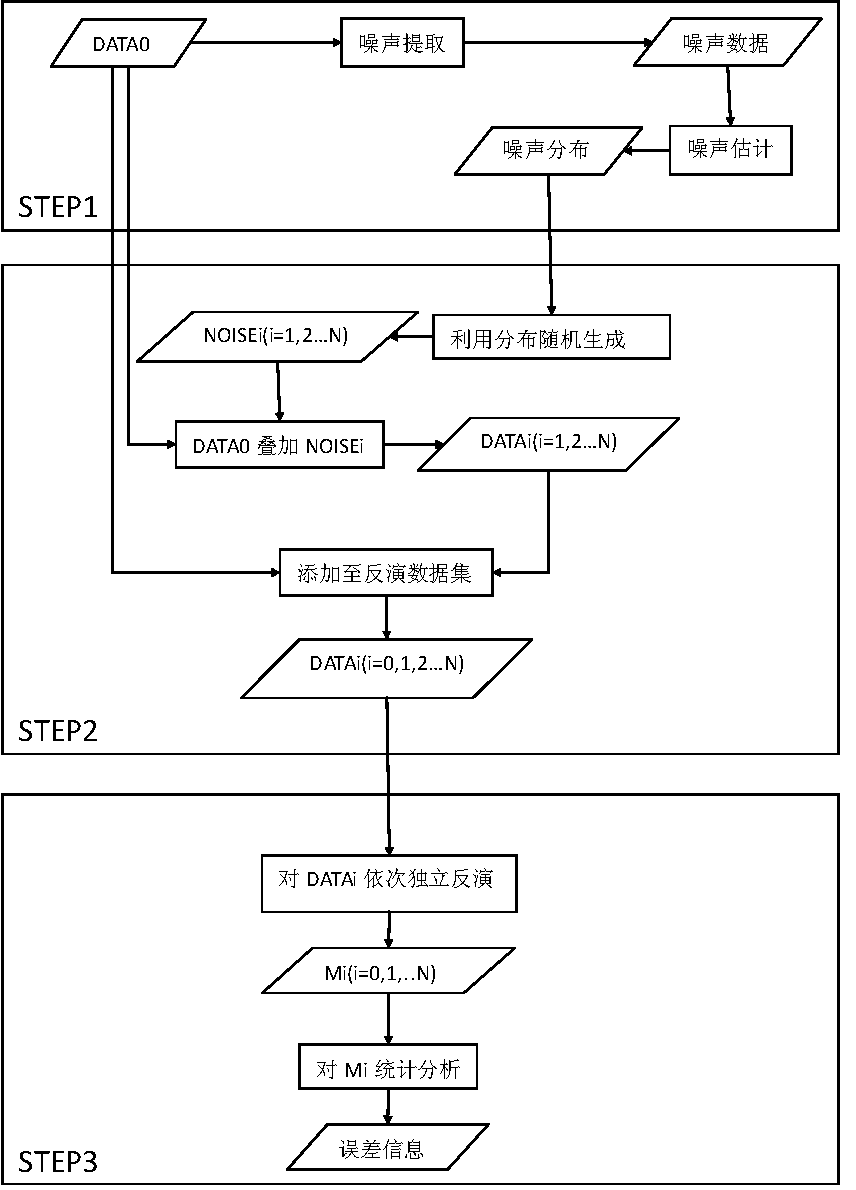
\includegraphics[scale=0.58]{fig2_03.pdf} 
  \caption{(a)不同震中距相对误差的分布,(b)(c)(d)分别为噪声、相对误差及波形振幅与震中距关系及统计回归线(虚线)}
  \label{fig2_03}
\end{figure}

CPS和CAP的权重均用震中距的函数进行计算定值,这主要考虑到地震波有衰减和几何扩散效应,随着震中距增大波形的振幅会减小,从而数据信噪比也降低。但实例计算发现简单的函数难以精确描述波形振幅或信噪比与震中距的关系,本文以2013年芦山地震未经滤波处理的远场地震波数据为例,计算分析信噪比及振幅随震中距变化的情况。首先假设P波之前的噪声数据为该台站观测数据的噪声平均样本,并设其为高斯白噪声,我们分别用观测波形的标准差($WaveStd$)和噪声的标准差($NoiseStd$)来衡量其振幅强度,并用它们的比值$NoiseStd/WaveStd$评估数据的相对误差。计算得到波形相对误差随震中距变化的关系如图\ref{fig2_03}(a)所示,可以看到相对误差随震中距变化比较散乱。为了使图像更直观展示相对误差随震中距的变化趋势,图\ref{fig2_03}(c)对图\ref{fig2_03}(a)中数据点进行最小二乘线性回归分析,将数据点进行连线并用虚线表示其回归直线,可以发现相对误差随着震中距增大而明显增加,表明信噪比确实随着震中距增大而降低。另一方面,如图\ref{fig2_03}(d)所示,地震波传播的几何扩散效应导致波形振幅强度随着震中距增大逐渐降低。

虽然上述的线性回归分析表明震中距与波形的信噪比或者振幅存在一定负相关性,但从图\ref{fig2_03}(c)和(d)中也明显看到相对误差和波形振幅强度随着震中距单调趋势变化过程中均有着不可忽视的波动性,导致它们与震中距的关系难以用简单的初等函数进行描述。这主要是因为波形振幅不仅仅由震中距完全决定,地下浅层结构的复杂性等因素也会对振幅造成难以估计的影响,所以尽管图\ref{fig2_03}(b)所示的随机噪声强度随震中距变化一直较平稳,但是作为波形噪声与振幅比值的相对误差却如图\ref{fig2_03}(c)所示有很大的波动性。综上分析,通过震中距的函数计算得到的信噪比或振辐调节权重因子是粗糙的。此外参考函数的具体确定也有较强主观性,如\citet{Zhu1996}通过震中距估计振幅变化幅度时,使用的估计公式中$r_0,p$参数经常通过经验进行赋值,其具体数值就可能因人而异。鉴于以上两个原因,本文舍弃用震中距表示权重的方法,而利用每道波形本身的数据信息直接进行针对性定权,对数据处理后的每道波形,用前文标准差比值的方法评估相对误差$RelativeError$,并设$|1-RelaitveError|$为信噪比权重因子$W1$,用波形的$L2$范数$L2norm$估计平均振幅,并构造表达式$1/L2norm$作为振幅调节权重因子$W2$,最终权重$WT$即定为$(1-NoiseStd/WaveStd)/L2norm$。

\section{误差评定方法}

\subsection{理论依据}
由于本文主要研究观测数据噪声导致的反演结果误差,首先分析观测数据噪声与反演结果的关系。为简单描述,以离散的线性反演问题为例,该案例引用自课程讲义\citep{zhu2009},详细推导证明可参考相关资料。设待求解矢量$m$与观测数据矢量$d$的关系为\refeq{eq2_17},其中$A$为参数矩阵,$\epsilon$为观测数据的随机噪声矢量。
\begin{equation}
\label{eq2_17}
	Am+\epsilon=d
\end{equation}

对\refeq{eq2_17}求解得$m$的估计量$\tilde{m}$,并进一步推得$\tilde{m}$的误差为\refeq{eq2_18},其中${\triangle}d$与${\triangle}\tilde{m}$表示相应量与期望的偏差。
\begin{equation}
\label{eq2_18}
	\triangle{\tilde{m}}=A^{-g}{\triangle}d
\end{equation}

假设对以上离散线性反演问题进行多次独立重复观测并反演的实验,则\refeq{eq2_18}变换可得到\refeq{eq2_19},其中“$\left \langle \right \rangle$”表示大量重复实验并统计。
\begin{equation}
\label{eq2_19}
	\left \langle \triangle{\tilde{m}}(\triangle{\tilde{m}})^T \right \rangle=
	A^{-g}\left \langle {\triangle}d({\triangle}d)^T \right \rangle  (A^{-g})^T
\end{equation}

接下来利用概率论和统计学原理,当重复独立实验的次数足够多,且在局部线性近似则关于$m$的协方差矩阵${\delta}m({\delta}m)^T$可近似表示为\refeq{eq2_20}所示。
\begin{equation}
\label{eq2_20}
	{\delta}m({\delta}m)^T \approx \left \langle \triangle{\tilde{m}}(\triangle{\tilde{m}})^T \right \rangle
\end{equation}

根据\refeq{eq2_19}可知,概率统计意义上,关于待求解量$m$的协方差信息完全可由多次观测数据的噪声${\triangle}d$计算得到。本文震源机制反演采用全局格点搜索方法,属于非线性反演。但是只要将\refeq{eq2_17}描述的问题一般化,仍然可以推得非线性反演中对应\refeq{eq2_19}的类似公式,待求解量$m$的协方差矩阵仍然可由大量具有不同偏差${\triangle}d$的$d$对应的解经统计得到。

基于以上原理,尝试在震源机制格点搜索反演中提出具体方案,对震源机制的误差进行评价。通过上面分析可知对应于一个包含数据噪声$\epsilon$的观测数据$d$可格点搜索计算出一个$\tilde{m}$,因此多个包含不同数据噪声$\epsilon$的样本$d$即对应了大量$\tilde{m}$,对其进行统计分析即可得到$m$协方差矩阵的估计值。

上述方案的关键点在于如何得到大量不同但合理的数据噪声$\epsilon$,然后计算大量对应的$\tilde{m}$用于估计${\triangle}\tilde{m}$。在现实观测中,通常$\epsilon$都近似符合高斯分布,因此只要事先分析得到$\epsilon$的概率分布函数,便可人工生成任意多的随机噪声$\epsilon$。在本文将每一个新生成的波形噪声$\epsilon$叠加上原始观测波形$d$,便得到了新的具有不同${\triangle}d$的$d$,将其独立用于格点搜索反演便能计算得到对应的一个新的$\tilde{m}$。大量重复该过程便依次得到了许多的$\tilde{m}$,然后利用\refeq{eq2_20}可估计其误差信息。

\subsection{方法步骤}
在实际震源机制格点搜索反演时,得到震源机制误差评价的过程主要分为三大步,具体可参考如图\ref{fig2_04}所示的流程图。
\begin{figure}
\centering
  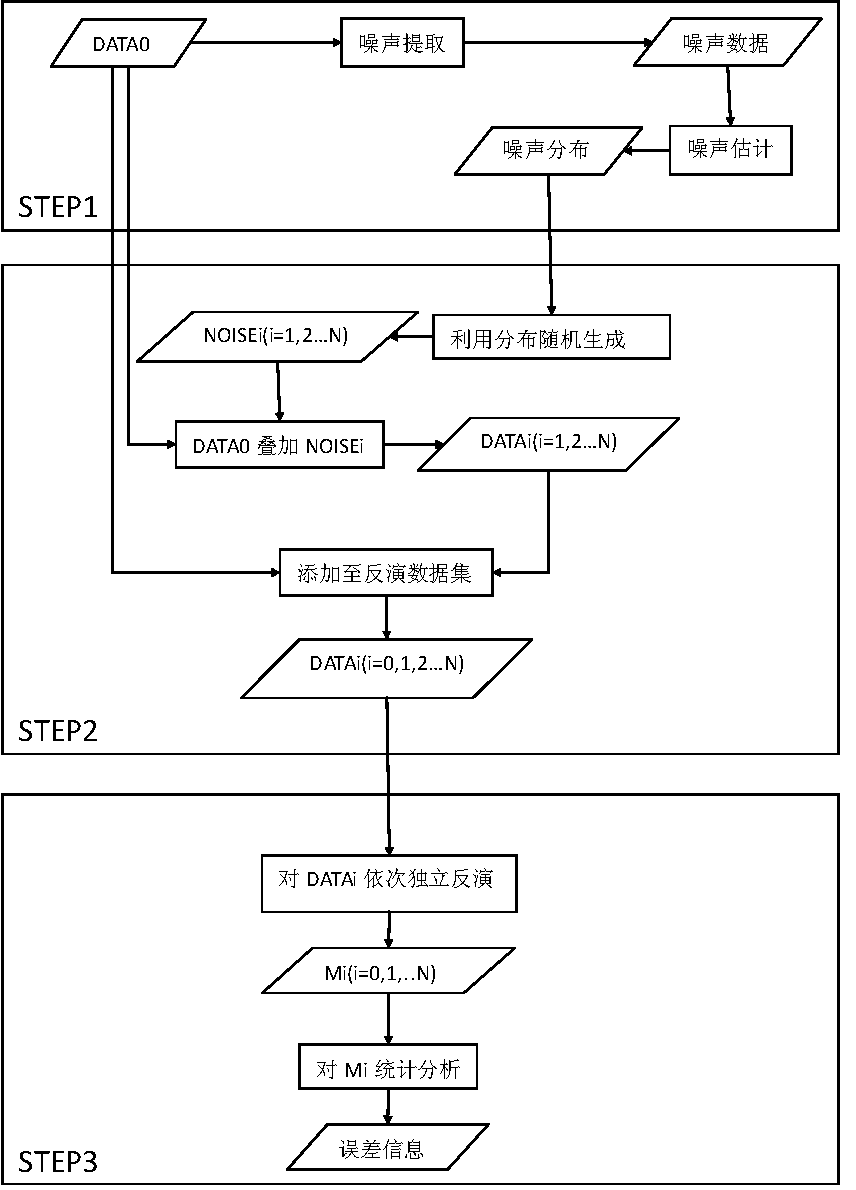
\includegraphics[scale=1.0]{fig2_04.pdf} 
  \caption{本文误差评定方法详细流程}
  \label{fig2_04}
\end{figure}

\begin{description}
\item[STEP1]数据噪声评估:估计出DATA0随机噪声分布,供之后完成数据模拟使用。
\begin{enumerate}
\item 提取原始观测数据DATA0中的纯噪声数据,首先假定在台站接收特定地震事件所激发波形的那段时间,台站附近的噪声是相对稳定的(接收特定事件波形很短,一般噪声不会突发变化),这样可以截取地震波首波到达前的一段数据作为该期间的纯噪声样本。
\item 估计噪声概率分布函数,将仪器接收到的噪声序列视为高斯白噪声(大量随机因素导致的误差总和常可做此近似),通过对地震波到达该台站前所记录的噪声序列样本进行参数估计,获得高斯分布的期望和方差,便得到了各台站数据噪声对应的概率分布函数$F(x)$。
\end{enumerate}

\item[STEP2]模拟数据:利用噪声分布函数$F(x)$以及原始数据DATA0生成模拟数据。
\begin{enumerate}
\item 生成模拟噪声,根据$F(x)$函数随机生成噪声,对应DATA0中各道波形的时窗长度和采样间隔分别生成同样采样点数的随机噪声,将包含各台站波形等时窗长度的噪声集合记为NOISE1,独立重复该噪声生成过程,可依次得到N个随机噪声集合的样本NOISE1、NOISE2...NOISEN,任一个噪声样本NOISEi(i=1,2,3..N)中均包含有对应于全部观测台站的随机噪声。
\item 进行模拟数据生成,以DATA1为例,将NOISE1中的噪声数据和DATA0中对应台站分量的原始观测数据相互叠加,便合成了对应于各台站的一套新波形数据,将其记为模拟数据DATA1,一般化以上过程,依次将NOISEi(i=1,2,3..N)分别加回到原始数据样本DATA0,便生成了包含合理随机噪声的N套数据样本DATA1、DATA2...DATAN。这N套模拟数据加上原始数据DATA0一起够成反演数据集。
\end{enumerate}

\item[STEP3]震源机制误差估计:计算大量震源机制并用概率统计评估。
\begin{enumerate}
\item 将每个数据样本DATAi(i=0,1,2,3...N)作为原始“观测”数据,分别独立通过格点搜索算法反演震源机制,得到误差范围内随机分布的震源机制M0、M1、M2...MN,所有Mi(i=0,1,2,3...N)组成了一个解集样本,样本容量即为总反演次数N+1。
\item 由统计学原理,当N足够大,且该解集样本包含的震源机制随机性足够好时,则解集样本的分布情况可以描述原问题中震源机制的误差情况。计算该样本的协方差即得到了震源机制的协方差估值。
\end{enumerate}

\end{description}
 %第二章 原理分析
%---------------------------------------

%%% Local Variables:
%%% mode: latex
%%% TeX-master: t
%%% End:

\chapter{理论实验}

\section{实验设定说明}
检验本文提出的权重优化方案和误差估计方法的有效性,关键是要看最终反演的震源机制是否为“真实”的震源机制,以及最终结果对数据随机噪声的反应,即误差大小。

为了能事先知道“真实”的震源机制,从而检验本文方法的有效性,设计了一个理论实验。本实验设置了一个Mw6.5级,震源深度为17km的地震,其震源机制为走向250°,倾角40°,滑动角82°,该参数设置的一个考虑因素在于与之后的应用实例,便于将结果进行相互比较。在ak135地球结构\citep{Kennett1995}下用波数积分法计算了震中距为4500km的8个台站的理论波形,为使方位分布满足约束要求,8个台站方位角分别选定为0°、45°、90°、135°、180°、225°、270°、315°。为方便述,将方位角从小到大的台站依次称为STA1、STA2、STA3、STA4、STA5、STA6、STA7、STA8,其分分布如\reffig{fig3_01}所示。
\begin{figure}
\centering
  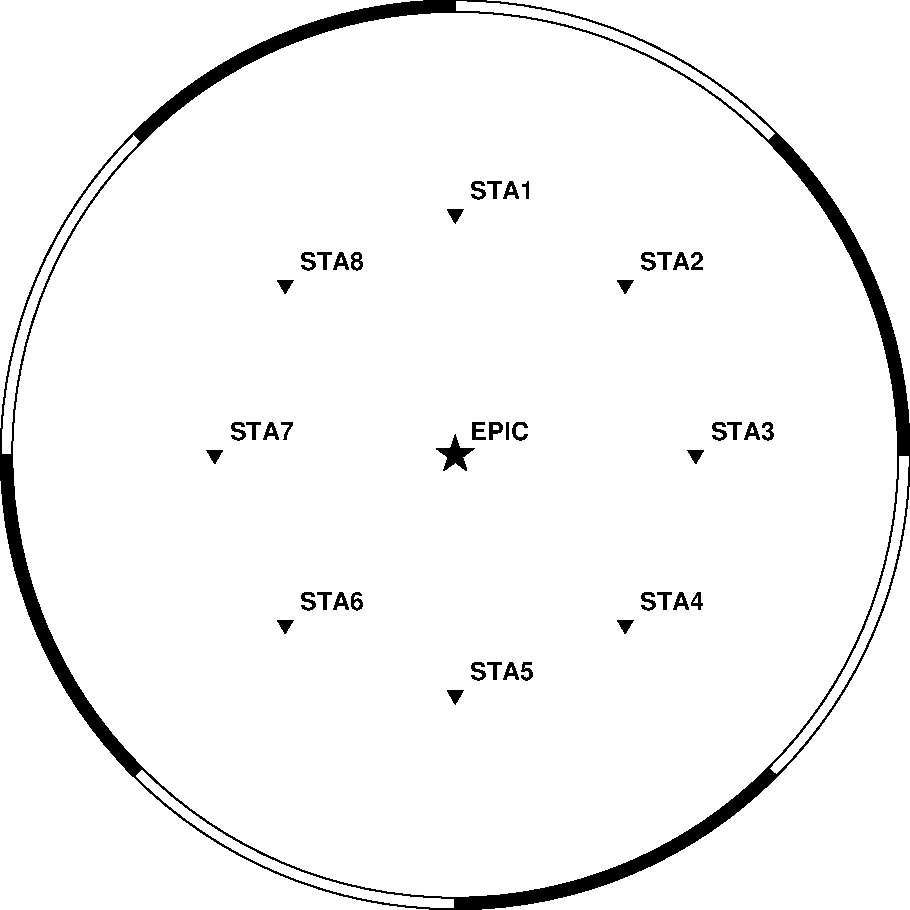
\includegraphics[scale=0.5,angle=0]{fig3_01.pdf}
  \caption{理论实验的台站分布,其中五角星表示震中,倒三角表示台站}
  \label{fig3_01}
\end{figure}

为了保证实验条件设定的合理性,首先要求满足原始数据对反演有足够约束力度。理论计算的原始无噪波形如\ref{fig3_02}所示,对于无噪数据,信噪比已经最大化,加权以及滤波等处理并不会影响反演结果。直接利用之后使用的P,S联合反演方法对该理论波形进行反演,结果与设定的震源参数完全一致,且拟合度为1(最高值,代表完全拟合),表明给定的数据结构具有反演该地震的能力,且计算机内离散化和数值舍入误差的影响可忽略不计。
\begin{figure}
\centering
  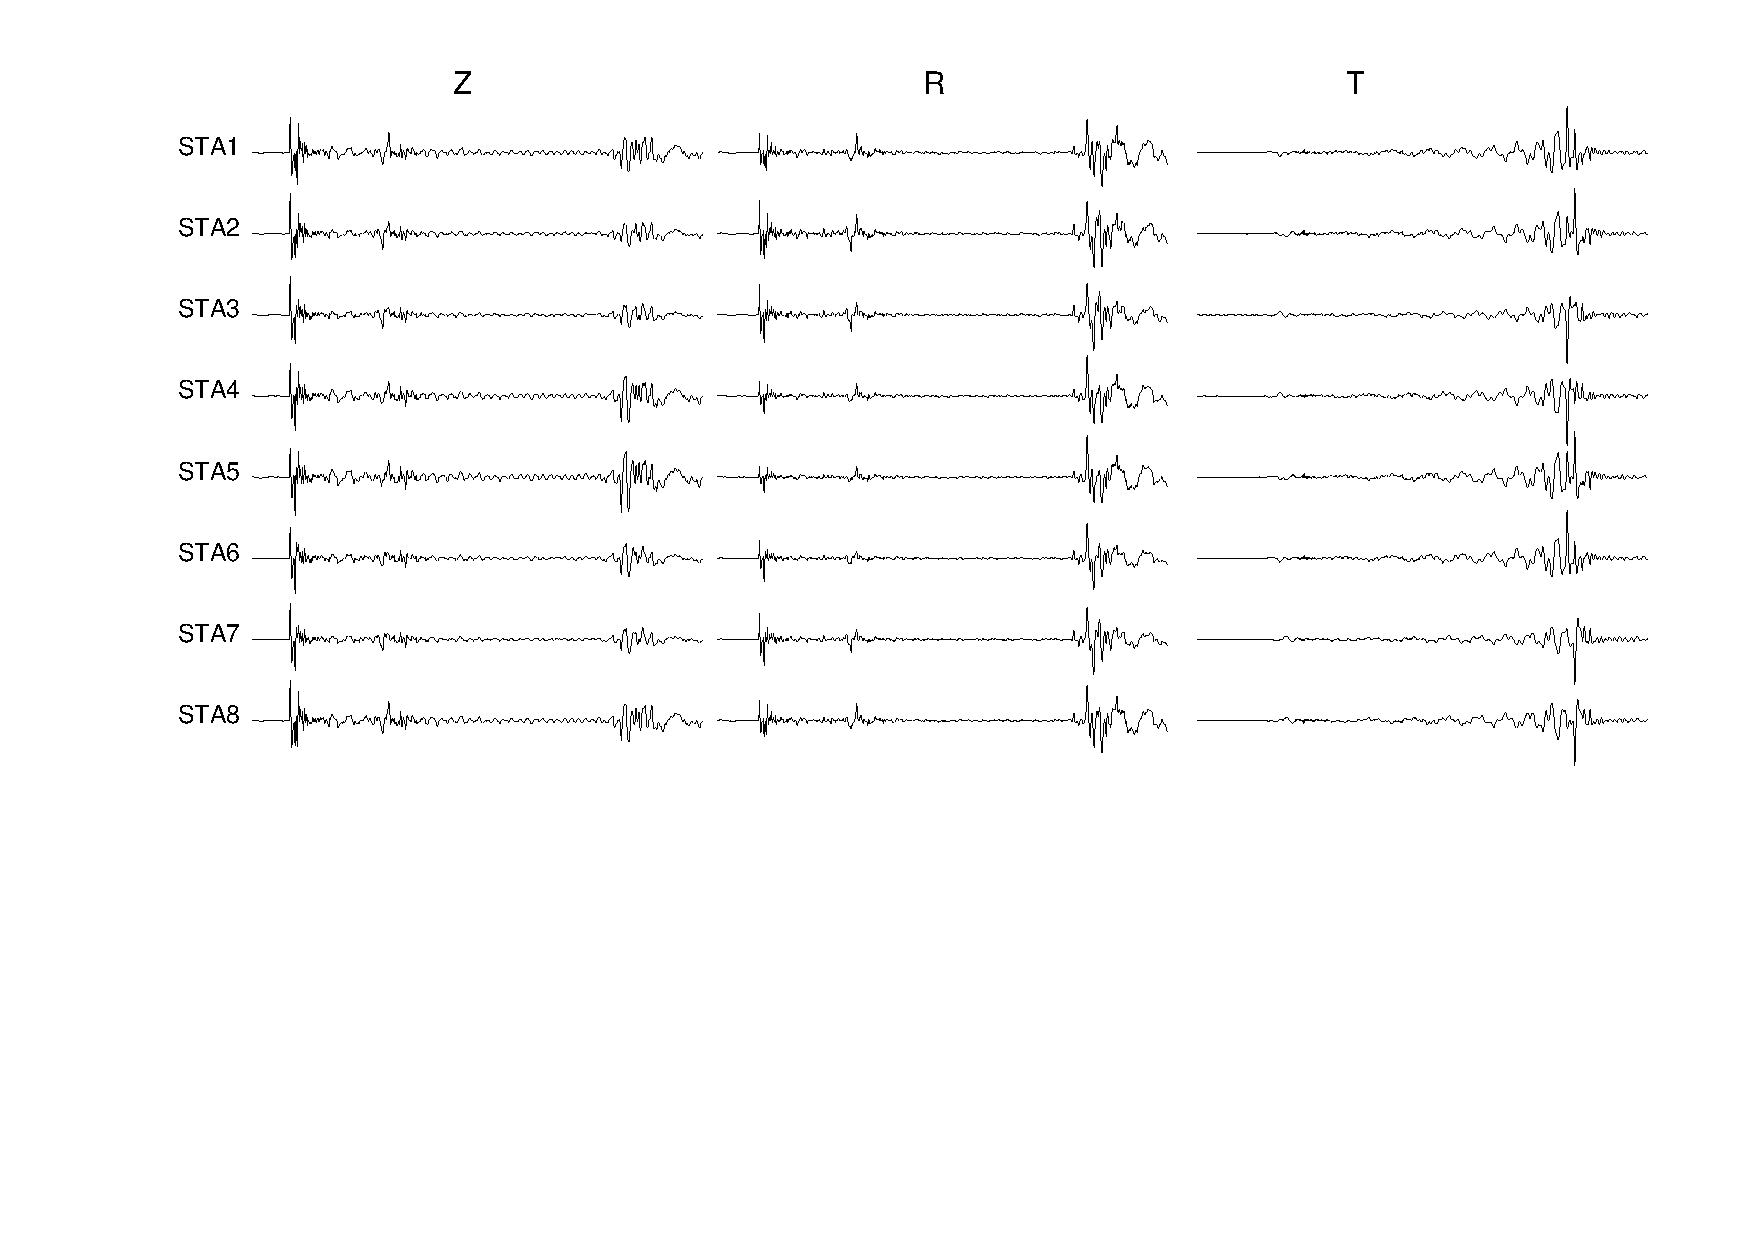
\includegraphics[scale=0.5,angle=0]{fig3_02.pdf}
  \caption{理论实验中通过波数积分法计算的各台站理论波形}
  \label{fig3_02}
\end{figure}

\section{权重优化检验}

\subsection{不同加权反演测试}
本文提出的权重优化方案是基于前人单独考虑振幅比加权或信噪比加权的方法,为了实际检验联合加权是否如理论分析一般对反演结果有优化作用,设置了一组对照实验用于检验。一共分为3组对照组,均采用以上章节理论实验相同的事件以及数据。但为了体现信噪比权重的作用,将原始噪声设置为高等强度,重复次数参数N设置为100,用P波和S波联合反演,以体现振幅比权重在不同振幅调节的作用。

三组对照组反演得到的结果如\reftab{tab3_01}所示,本实验仍旧使用了之前一样的方位分布较好的台站,可以发现即使在数据结构较好的情况下,使用完全一样的反演数据,以及同一反演程序,三组反演的结果还是有可见差异的。经过不同加权反演后,虽然结果均离真值偏差不大,但明显可以看到,W1加权拟合度最高,因为它尽可能抑制噪声影响,降低高噪声数据权重,以追求整体数据的最大拟合度,其震源机制也与真值较接近,但震源深度却与真实深度偏差了1km。而W2虽然由于没有经过信噪比加权,拟合度在三组中最差,可震源深度却没有明显偏差,不过震源机制比W1略差。而对于联合了W1与W2加权的WT加权反演组,由于同时考虑了数据信噪比以及数据不同振幅权重,其拟合度情况不致于太低,而且综合来看震源深度和震源机制更接近真值(虽然差异不大,但毕竟是完全一样的反演数据)。
\begin{table}[ht]
\centering
\caption{三种加权方案得到的解}
\label{tab3_01}
    \begin{tabular}{c c c c}
    \hline
     & 走向/$\degree$ & 倾角/$\degree$ & 滑动角/$\degree$ \\
    \hline
    真值		& 250 & 40 & 82  \\
    W1		&  &  &  \\
    W2		&  &  &  \\
    W3		&  &  &   \\
    \hline
    \end{tabular}
\end{table}

针对以上反演结果进行深入分析,数据主要包括P波和S波数据,这两震相数据所加的噪声强度是一致的,而在纯剪切位错源情况下,所激发的S波震相的振幅要明显高于P波振幅。因而两种数据中,S波的信噪比相对较高,且振幅更大。众所周知,与P震相接近的远震pP及sP震相对震源深度具有较好的约束作用,而它们已经包含在反演所截取的P波时窗中,也即P波数据对震源深度约束效果比较强。考虑到波形中所加的噪声是随机白噪声,其高度随机性决定了它基本不可能被理论波形拟合。所以噪声在干扰反演结果的同时,也很明显地会降低最终数据拟合度,因而拟合度Fit暗示了噪声对结果的干扰程度,是结果可信度的象征。对W1信噪比加权反演组,对高信噪比的S波赋予了较大权重,加之S波本身的高振幅更使得反演中S波数据对反演结果占主导作用。P波的贡献被减弱,因而P波的深度约束没能很好体现,最终导致其结果拟合度在三组对照组中最高,其深度却偏差最大。对于W2加权对照组,进行了振幅调节加权,振幅大的S波权重相对削弱,使P波获得了同等影响力,然而却忽略了P波信噪比较低,P波中占比较大的噪声也在反演中对结果起到了消极的干扰作用,理所应当拟合度会相对较低,虽然深度得到了较好约束,但噪声干扰也可能对结果有一定影响。最后,联合信噪比和振幅调节的WT加权反演组,没有过分强调追求拟合度,合理调节振幅分配了权重,使得不同振幅震相均在反演中起到了相对平等的作用,另一方面由于W1权重的特性还在一定程度上压制了高噪声对震源反演的干扰。反演结果的拟合度虽比W1略有所降低,但更多的有用信息使得对震源机制和震源深度的约束作用更强,并且结果受噪声的随机扰动影响也可能更小,结果更为稳定。

以上分析说明信噪比和振幅调节联合加权确实相对于其单独加权更合理,在反演时能在一定程度上优化结果,WT加权得到的反演结果综合来说更可靠、准确地反映了真实情况。

\section{误差评定检验}

\subsection{理论实验反演过程}
真实情况下的数据都是有噪声的,这也正是本文误差评价所关心的误差来源。本文采用高斯白噪声给理论波形加噪,以模拟最原始的“观测”数据。将加了随机产生的高斯白噪声的理论波形视为台站处接收到的“观测波形”,为方便描述,将该套数据整体记为DATA0。

利用本文的误差估计方法法对震源机制进行反演并估计误差完全的步骤如下:1.首先估计原始噪声,用参数估计方法对DATA0中每道数据波形分别估计其噪声的强度,估计时选取P波到达前的空白震相期波形作为该道波形的噪声数据样本,并将其视为符合高斯分布的序列,从而可利用参数估计得到该噪声分布的标准差;2.而后模拟等价噪声,利用上一步得到的DATA0中各道波形噪声的标准差分别生成与原波形时窗长度相等的高斯白噪声序列;3.生成模拟带噪数据,并上步生成的高斯白噪声与DATA0中各道波形按噪声标准差对应相加,便得到了第一套模拟带噪数据DATA1;4.生成多套模拟数据,重复步骤2,3,每重复一次可得到一套新的模拟带噪数据,假设一共重复N次,便得到DATA1,DATA2...,DATAN,总共N套模拟数据;5.重复反演得到解集,对原始观测数据和模拟数据中的每套数据DATAi(i=0,1,2..N),采用同样的数据处理方式和权重方案,分别利用CPS程序进行独立反演,得到的对应的震源机制解Mi(i=0,1,2,...N);6.统计解集得到误差信息,利用统计方法对Mi(i=0,1,2...N)样本进行估算得到均值、协方差及相关系数信息。至此便在用“观测”数据反演得到震源机制M0的同时得到了M0各项参数的协方差等误差信息。

在理论实验的每次独立反演过程中,均采用同样的数据处理方式,并用震相中的P波与S波(SV,SH)进行联合反演。为了尽可能模拟真实情况,数据进行了时窗截取,噪声滤波等处理。P波数据截取了相对P波到时(-10s,30s)的时窗,并进行(0.01-0.1Hz)带通滤波;SH波滤波频率为(0.05-0.1Hz),时窗选为相对其震相到时(-20s,40s)的范围;SV波的波形与其它震相交叠延续,时窗设定较长,为相对到时(-30s,150s)范围。在格点搜索过程中为保证效率分步进行,第一步全空间快速搜索,步长为10度,第二步在上一步搜索的最优点附近进行局部精搜索,步长为1度。

\subsection{不同噪声强度测试}
由于反演公式复杂,而且反演数据量大,直接得到数据误差到反演模型的误差传播矩阵非常困难。因此在模拟实验中,给定数据误差的情况下,无法得到反演模型的误差期望,用于检验。故在误差方法的理论检验实验中,我们改变了将检验目标改为两个。一是检验理论真值是否在反演结果的误差范围内,这是最基本也最重要的要求;二是检验结果的误差大小是否与原始噪声强度有正相关关系,根据误差传播规模,最终的模型误差为误差传播矩阵与原始数据噪声误差之积。

为检验该两目标,分别设置多组对照组,每组的数据原始噪声强度大小不同,其余参数均一致。对照组共分为4组,各组噪声均为高斯白噪声,考虑到波形的振幅强度基本为$10^-5m$量级,将噪声标准差大小分别设置为低噪声组$1.0*10^-6m$,中噪声组$2.5*10^-6m$,高噪声组$5.0*10^-6m$,超高噪声组$1.0*10^-5m$,并将误差评价方法中重复反演次数N定为100。

向理论波形加入不同强度的高斯白噪声,生成的“观测波形”DATA0经搜索反演和本文误差估计,得到震源机制均值和误差中误差,具体结果如\reftab{tab3_02}所示。
\begin{table}[ht]
\centering
\caption{低强度噪声组误差协方差和相关性}
\label{tab3_02}
    \begin{tabular}{c c c c}
    \hline
    协方差 & 走向/$\degree$ & 倾角/$\degree$ & 滑动角/$\degree$ \\
    \hline
	走向/$\degree$ 		&1.0619 	&-0.0365	&0.5275\\
	倾角/$\degree$		&-0.0365	&0.1275		&0.0175\\
	滑动角/$\degree$	&0.5275		&0.0175		&0.707\\
    \hline
    \end{tabular}
    \begin{tabular}{c c c c}
    \hline
    相关系数 & 走向/$\degree$ & 倾角/$\degree$ & 滑动角/$\degree$ \\
    \hline
	走向/$\degree$ 		&1 			&-0.0991	&0.6085\\
	倾角/$\degree$		&-0.0991	&1			&0.0583\\
	滑动角/$\degree$	&0.6085		&0.0583		&1\\
    \hline
    \end{tabular}
\end{table}

\begin{table}[ht]
\centering
\caption{中强度噪声组误差协方差和相关性}
\label{tab3_03}
    \begin{tabular}{c c c c}
    \hline
    协方差 & 走向/$\degree$ & 倾角/$\degree$ & 滑动角/$\degree$ \\
    \hline
	走向/$\degree$ 		&5.7756 	&-0.2966	&3.7714\\
	倾角/$\degree$		&-0.2966	&0.5651		&0.3579\\
	滑动角/$\degree$	&3.7714		&0.3579		&4.9891\\
    \hline
    \end{tabular}
    \begin{tabular}{c c c c}
    \hline
    相关系数 & 走向/$\degree$ & 倾角/$\degree$ & 滑动角/$\degree$ \\
    \hline
	走向/$\degree$ 		&1 			&-0.1642	&0.7026\\
	倾角/$\degree$		&-0.1642	&1			&0.2132\\
	滑动角/$\degree$	&0.7026		&0.2132		&1\\
    \hline
    \end{tabular}
\end{table}

\begin{table}[ht]
\centering
\caption{高强度噪声组误差协方差和相关性}
\label{tab3_04}
    \begin{tabular}{c c c c}
    \hline
    协方差 & 走向/$\degree$ & 倾角/$\degree$ & 滑动角/$\degree$ \\
    \hline
	走向/$\degree$ 		&34.8539 	&-5.3033	&25.7959\\
	倾角/$\degree$		&-5.3033	&3.2651		&-4.6973\\
	滑动角/$\degree$	&25.7959	&-4.6973	&32.7579\\
    \hline
    \end{tabular}
    \begin{tabular}{c c c c}
    \hline
    相关系数 & 走向/$\degree$ & 倾角/$\degree$ & 滑动角/$\degree$ \\
    \hline
	走向/$\degree$ 		&1 			&-0.4971	&0.7634\\
	倾角/$\degree$		&-0.4971	&1			&-0.4542\\
	滑动角/$\degree$	&0.7634		&-0.4542		&1\\
    \hline
    \end{tabular}
\end{table}

\begin{table}[ht]
\centering
\caption{超高强度噪声组误差协方差和相关性}
\label{tab3_05}
    \begin{tabular}{c c c c}
    \hline
    协方差 & 走向/$\degree$ & 倾角/$\degree$ & 滑动角/$\degree$ \\
    \hline
	走向/$\degree$ 		&101.05 	&-1.0465	&101.852\\
	倾角/$\degree$		&-1.0465	&20.1075	&5.6095\\
	滑动角/$\degree$	&101.852	&5.6095		&141.257\\
    \hline
    \end{tabular}
    \begin{tabular}{c c c c}
    \hline
    相关系数 & 走向/$\degree$ & 倾角/$\degree$ & 滑动角/$\degree$ \\
    \hline
	走向/$\degree$ 		&1 			&-0.0232	&0.8525\\
	倾角/$\degree$		&-0.0232	&1			&0.1053\\
	滑动角/$\degree$	&0.8525		&0.1053		&1\\
    \hline
    \end{tabular}
\end{table}
考虑到搜索精度为1°,并假设误差范围不超过3倍中误差大小,则得到的最终反演结果和可能误差范围如\reftab{tab3_06}。
\begin{table}[ht]
\centering
\caption{加不同强度原始噪声得到的解及误差范围}
\label{tab3_06}
    \begin{tabular}{c c c c}
    \hline
    加噪强度 & 走向/$\degree$ & 倾角/$\degree$ & 滑动角/$\degree$ \\
    \hline
    无噪声		& 250 & 40 & 82  \\
    低噪声		& 250+3 & 40+3 & 82+3  \\
    中等噪声	& 250+8 & 40+3 & 83+7  \\
    高噪声		& 246+18 & 40+6 & 78+17  \\
    超高噪声	& 245+30 & 42+14 & 84+36  \\
    \hline
    \end{tabular}
\end{table}

利用模拟分析法得到的震源机制均值虽然使得三个参数都与真值出现了偏离,但是却给出了误差信息,而且不难发现均值与真值的偏差都在三倍估计标准差内,说明估计是有效的。此外,从\reftab{tab3_02}中的三个参数间相关系数可以发现,在此反演中三间是有较强相关性的。相关系数的符号暗示了受到噪声影响时,在统计意义上震源机制三个参数间变化趋势的关系。标准误差估计了数据随机噪声引起的震源机制偏差大小,而相关系数则预测了震源机制各参数受扰动时的模式,而非是杂乱无章的。

从反演结果可以看出,在不同噪声强度的对照组中,所给出的最终结果的误差范围内均包含真值——走向250°,倾角40°,滑动角82°,验证了本实验的第一个目标——有效性。而从随机性角度,一次反演的结果可能在误差范围内取任意不可预料值。各组实验均有不同程度的误差,表明即使用信噪比较高的,数据结构分布很好的优质数据作为输入数据,反演时得到的结果仍然可能与真值有一定偏差。实验显示,在格点搜索反演震源机制时,即使较低数据随机噪声的影响仍然不可忽略,表明了误差分析在的必要性。

另一方面,随着原始数据噪声逐渐增强,即使数据经过滤波提高信噪比,其反演结果的均值与真值偏差也倾向于越来越大。但同时,估计的误差范围也伴随着增长,仍然保证了真值在误差范围内。误差大小与数据噪声基本保持了正相关的趋势,符合关于误差性质检验的第二个目标。随着反演结果的误差逐渐变大,精确度变低,其参考性和科学意义也随之降低。如在本实验中,噪声强度和有效波形振幅相当的超高噪声情况下,震源机制误差已经高于30°,基本超出了参考应用的可接受范围,科学价值很低。该结果体现了原始数据对于反演结果的重要性,原始数据质量决定了最终结果的优劣。 综上,本次不同噪声强度的对照实验表明本文误差估计方法可靠,其有效地反映了不同数据随机噪声对反演结果造成的误差。在震源机制的格点搜索反演中,即使高信噪比数据中噪声造成的误差也超过了搜索精度,不可忽略。由于原始数据质量从根本上决定了最终结果好坏,及包含的科学意义,在实际工作中应该筛选优质观测数据,及时剔除不可靠或劣质数据。为了吻合真实观测数据的信噪比,后续理论反演中将噪声强度设置为中等强度,即$2.5*10^-6$m。

\subsection{不同反演次数测试}
在本文的误差评价方法中,主要利用随机统计原理,需要进行多次重复反演,其中反演次数N为人为设定。从统计学理论知道,为了满足样本对全体估计的可靠度,要求样本具有随机性,且样本容量不能过小。在本文的误差评价方法中,每一次重复反演时,均对数据的每一道波形的每一个采样点的噪声进行了随机生成,保证了统计要求的随机性。而每一道波形包含了大量的采样点,数据全体有不同台站不同分量的多道波形,因此总采样点数很大,以满足噪声影响统计时原始噪声的样本容量大小。为了确保重复反演次数设置合理,使误差统计方法生效,设置对照组分别对应不同重复反演次数N,并对比实验结果。总共设置了5组对照组,分别将重复反演次数N设置为20,40,60,80,100。

为了方便对比不同参数N的结果,以分析不同N对结果的影响,确认设置的N参数合理,将各对组结果统一列入\reftab{tab3_07}中。
\begin{table}[ht]
\centering
\caption{不同重复反演次数N对应的解及误差范围}
\label{tab3_07}
    \begin{tabular}{c c c c}
    \hline
    反演次数 & 走向/$\degree$ & 倾角/$\degree$ & 滑动角/$\degree$ \\
    \hline
    真值		& 250 & 40 & 82  \\
    \hline
    \end{tabular}
\end{table}

从表中可以看出,各组反演结果的误差的三倍中误差范围内均包含理论真值,表明各反演对照组结果均准备可靠。在大量采样点噪声随机生成的保证下,不同反演次数的结果基本一致,体现了反演样本具有很高的随机性。在如此高随机性条件下,统计结果对总反演次数N不是很敏感。随着N的要求降低,可以有效减少重复计算带来的计算压力,应用中可根据实际情况和硬件能力考虑N的取值。为了更大程度保证结果可靠性,本文的后续计算中均将重复反演次数N设置为100。
 %第三章 理论实验
%---------------------------------------

%%% Local Variables:
%%% mode: latex
%%% TeX-master: t
%%% End:

\chapter{实例应用}

\section{案例选取}

为了验证本文联合定权方案和误差评定方法的实用性,将其应用到芦山地震中实际反演其震源机制和误差信息。芦山地震发生于2013年4月20日,震级超过$M_w$6级,震源中心在四川省雅安市芦山县附近,是继2008年汶川特大地震以来龙门山断裂带发生的又一强震。地震发生后造成几百人死亡,上万人受伤,受灾人口超过200余万\zhcitep{崔鹏}{cuipeng2013},引起了社会各界关注。在直接造成特大地震灾害的同时,芦山地震还诱发了大量的次生地质灾害,其中主要包括落石、崩塌、堰塞湖、泥石流、滚石和滑坡等\zhcitep{陈晓清}{chenxiaoqing2013}。这些次生灾害造成的人员伤亡和经济损失也十分巨大,不低于地震的直接影响。

从科学研究的角度看,选取该地震进行方法应用,反演其震源机制有以下两方面优势:首先,芦山地震$M_w$震级在6-7级之间,既可以保证足够的远场地震波能量,同时又可避免过大震级的震源复杂性对波场影响;其次该地震发生后,引起了大量学者的关注,并对其震源机制做了许多研究,有非常多结果可用于与本文方法反演的震源机制进行参考对比,检验结果的可靠性。

\section{反演方案}
反演基于CPS程序的Fit互相关拟合目标函数,利用格点搜索算法进行全空间搜索寻找最优解。为了排除参考震源深度的误差影响,在反演过程中将震源深度也设为可变量,同时加入反演范围。在格点搜索反演中,将震源深度的搜索步长设为1km。而震源机制的搜索则细分为两步,第一步进行全空间快速搜索,将走向、倾角、滑动角的搜索步长均定为10$\degree$,保证求解收敛过程不会陷入局部最优的同时还保证了较高的搜索速度,第二步则进行区域内精搜索,将走向、倾角、滑动角的搜索步长均定为1$\degree$,通过局部范围的少量搜索计算,将最优震源机制的精度提升至1$\degree$。

应用本文误差估计方法评价震源机制误差时,直接将下载的去除仪器响应后的台站数据视为DATA0,然后按照估计方法的流程图进行操作。由于真实地震的震源机制是未知的,不可能像理论实验中比较真值与误差范围的关系一样检验误差是否准确。在此,我们将本地震的误差结果与理论实验的估计误差进行比较、相互印证。之所以可以相互印证是因为刻意设置使得两地震的震源机制相似,虽然使用的观测数据不同,其误差绝对大小也会不同,但是同类型地震各参数间的相关性,以及不同参数的稳定性大小应该是相近的。

为了检验本文提出的WT联合权重在实际应用中的优化效果,设置了三组对照组,分别尝试用WT联合加权、单独W1信噪比加权和单独振幅调节加权W2三种定权方案,对芦山地震的震源机制独立进行反演,并将结果比较分析。对三种加权方案对照组的反演结果评比时综合考虑其结果的稳定性和可靠性。稳定性主要比较反演结果的拟合度高低和震源机制的误差大小。而评价可靠性时,由于无法得知芦山地震震源机制的真值,转而间接考虑可靠性的反面——多解性。如果反演中最优解与其它解差异明显,则表示该解较显著,且有唯一性,较可靠。相反,如果反演过程中搜索到多个极值或性质相近的点,说明具有多解的可能性较大,解不可靠。

\section{数据处理}

在本案例反演过程中,考虑到远震SV波受到其后续波SPL(shear couple wave)的影响,而SPL对地壳上地幔结构敏感,不利于拟合反演,故放弃了SV波,选用远场台站波形中体波P震相和SH震相数据进行震源机制反演。

我们仅使用了远场体波数据,一方面是因为近场波形反演对震源区局部的浅层结构误差敏感,根据\zhcitet{郑勇}{zhenyong2013}和\zhcitet{高原}{gaoyuan2013} 的相关研究,发现芦山地震恰巧位于地壳厚度和波速结构横向变化剧烈之处。\zhcitet{谢祖军}{xiezujun2013}的研究更直接表明不同一维模型对芦山地震近震反演的震源参数影响高达到10°,而远场波形则对地壳及上地幔的横向非均匀性和震源破裂细节的复杂性不敏感,因而远场数据相对于近场数据更合适于该地震的震源机制反演中。 
另一方面,在前文中提到体波相位的系统性误差理论上可通过平移因子K来抵消,但面波具有频散效应,使得K因子无法很好地补偿结构误差对其相位的影响,且面波易受浅层结构横向非均匀性影响,基于以上考虑,反演时舍弃了面波数据。

在远震情况下,随着震中距增加,地震波的穿透深度越来越深。当震中距接近98$\degree$时,地震波传播路径到达核幔边界,这时将产生绕射波$P_d$,其影响范围如\reffig{fig4_01}所示非常广\citep{Stein2003},但基本在震中距大于98$\degree$的区域。此外,由于核幔边界处的折射作用,在震中距为98$\degree$-145$\degree$的范围内,没有直接穿透的地震波能量到达,该范围内主要受绕射波影响比较大。绕射波在核幔边界的临界条件下产生,对地下结构非常敏感,不适用于震源机制反演。另一方面,为了能将较大地震的破裂面当作点源处理,震中距也不宜太近。
\begin{figure}
\centering
  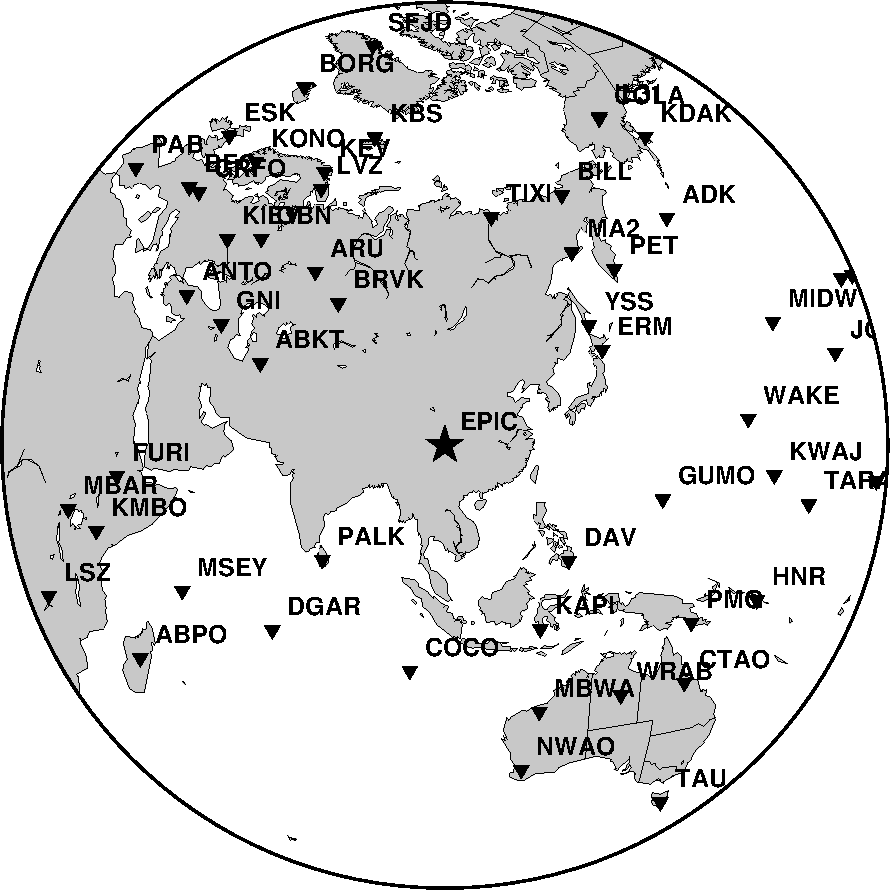
\includegraphics[scale=1.2]{fig4_01.pdf}
  \caption{随着震中距增大,远震情况下绕射波的产生\citep{Stein2003}}
  \label{fig4_01}
\end{figure}


据上分析,本文选取了IRIS提供的54个震中距在30°-90°之间且方位分布较均匀的地震台站(如\reffig{fig4_02}所示),利用这些台站记录的宽频带P波及SH波数据,以ak135模型\citep{Kennett1995}作为地球参考模型通过波形拟合反演震源机制。反演过程中经过多次数据挑选进行除错以提高数据信噪比,最终选取了信噪比较高的102道P震相波形数据和38道SH波波形数据。首先对下载的台站数据进行诸如去除仪器响应、方位旋转等预处理。然后对P波截取了相对P波理论到时(-10s,30s)的时窗,并进行(0.01Hz,0.1Hz)频率范围的带通滤波(该滤波范围基于频谱分析以及多次滤波试验选定)。对38道挑选的SH波数据进行数据处理时,带通滤波频率范围为(0.005Hz,0.06Hz),时窗则选为相对SH波理论到时(-30s,100s)的时间段。
\begin{figure}
\centering
  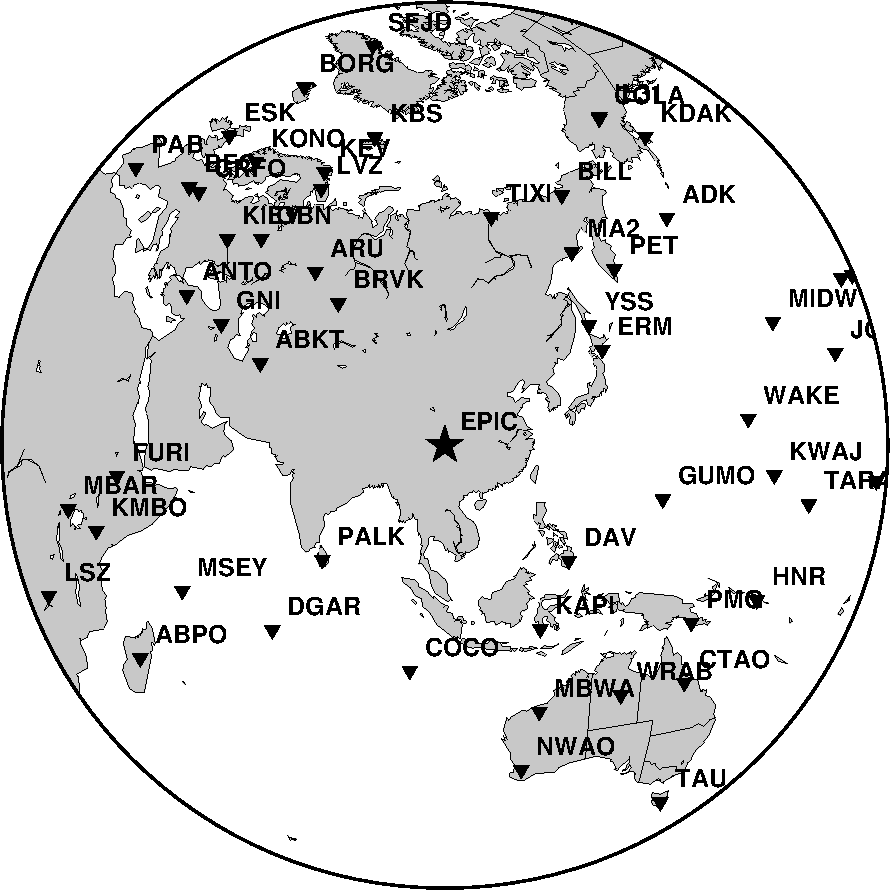
\includegraphics[scale=0.6]{fig4_02.pdf}
  \caption{波形反演所用数据的台站分布,其中五角星表示震中,倒三角表示台站}
  \label{fig4_02}
\end{figure}

\section{反演结果}
三组不同加权对照组反演的震源机制及深度等结果如\reftab{tab4_01}所示,总的来说三次反演结果均较一致,说明该数据分布较理想,结果较稳定,加权起到对反演结果的一种微调作用。
\begin{table}[ht]
\centering
\caption{三种加权方案反演芦山地震的结果}
\label{tab4_01}
    \begin{tabular}{c c c c c c c}
    \hline
    加权方案 & 深度/km  & 走向/$\degree$ & 倾角/$\degree$ & 滑动角/$\degree$ & 震级($M_w$) & 拟合度(Fit) \\
    \hline
    W1		& 16  & 202 & 47 & 96 & 6.49 & 0.7827 \\
    W2		& 18  & 213 & 41 & 95 & 6.41 & 0.5822 \\
    WT		& 17  & 211 & 41 & 94 & 6.41 & 0.6052 \\
    \hline
    \end{tabular}
\end{table}

简单来看,三组对照组中,W1加权组拟合度最高,WT联合加权组次之,而W2加权组拟合度最低。同样的,WT加权组的震源深度结果17km居于另两组震源深度之间,W1加权组和W2加权组的震源深度分别为16km和18km,均只与之相差1km(深度搜索精度为1km)。三组对照组反演的震源机制的三个参数中,走向的差异最大,倾角次之,而滑动角最相近,而从参照组整体来看,W2加权参照组与WT加权参照组的震源机制非常接近,而与W1加权反演组有较明显区别。

\section{分析讨论}
\subsection{结果分析}
首先分析三次反演的拟合度大小以体现W1的作用,从反演理论可知适当增加高质量数据的权重可以减小反演结果的误差,使结果更稳定,并使理论数据与观测值吻合得更好,提升最终的拟合度Fit。从\reffig{fig4_03}所示三组对照组拟合度随深度变化的曲线图,可以发现WT联合加权反演与W2单独加权反演的拟合度曲线非常接近,不过后者的拟合度始终略高于前者。这是因为WT加权反演时对数据信噪比进行了考虑,使得信噪比较低的波形数据在反演中的权重有适当下降,减弱了低信噪比数据中比重较大的随机噪声对反演结果的干扰,同时也使得预测数据与观测数据间的拟合度有所提升。同理,W1单独加权参照组的反演拟合度应是三个参照组中最高的,在\reffig{fig4_03}也能看到W1加权组的拟合度曲线明显高于其它两组。这也是因为W1加权反演组是基于数据随机噪声强度调节权重,为单纯追求反演的拟合度最高,压制了信噪比较低的数据在反演中的作用,而提高了高信噪比数据的贡献,使结果侧重于尽可能满足与高信噪比数据的吻合,最终拟合度也随之提升。此外,对于低振幅的震相,信噪比相对较低,进行W2振幅比调节放大低振幅震相的作用时,也进一步放大了其中的噪声影响,因此数据的整体信噪比会有所下降。因此包含振幅调节加权的两个对照组的拟合度会比W1加权组有较明显的降低,而WT联合加权组的拟合度会比W2加权反演组有所提高。三组反演对照组的拟合度相对大小情况,恰好符合三种加权方案的理论预期效果。
\begin{figure}
\centering
  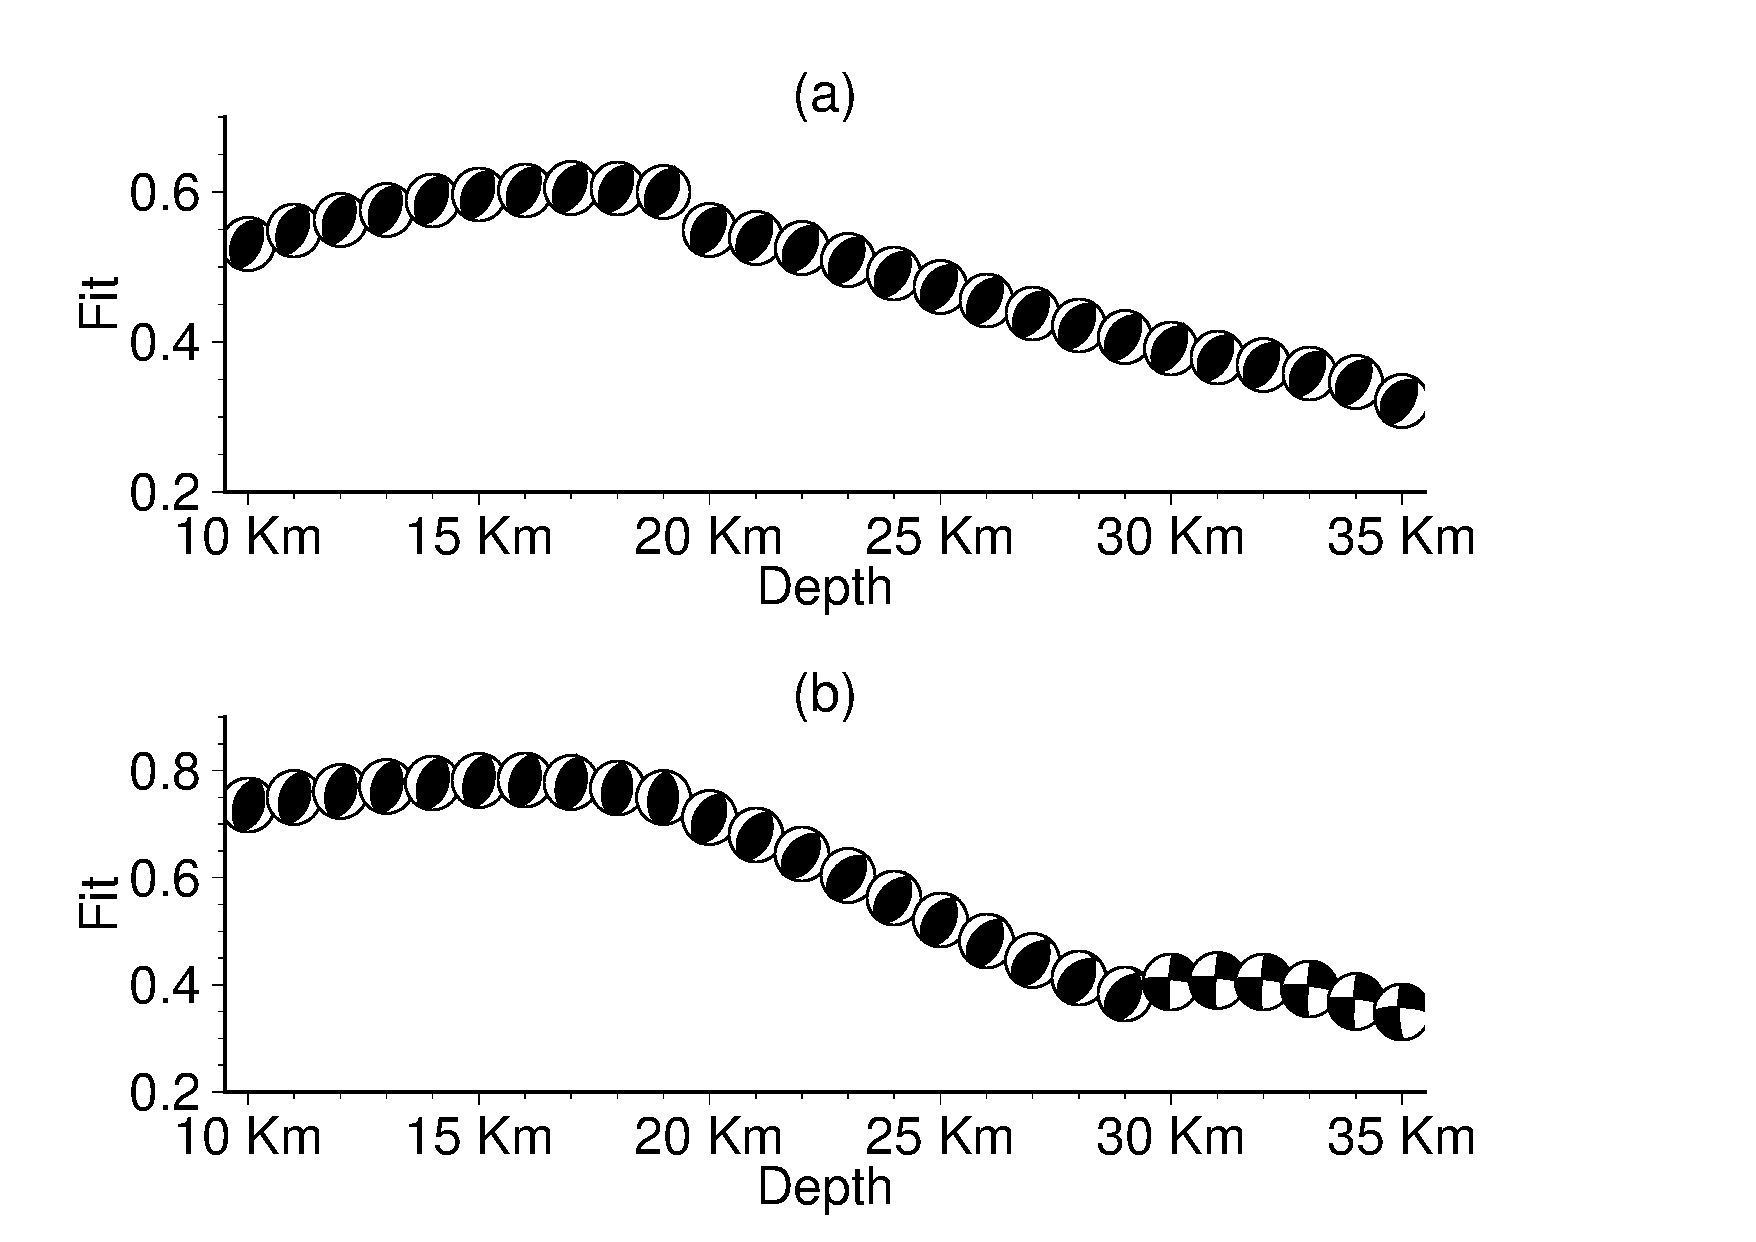
\includegraphics[scale=0.4,angle=0]{fig4_03.pdf}
  \caption{三种反演方案拟合度随震源深度的变化曲线}
  \label{fig4_03}
\end{figure}

前文理论分析中说明了拟合度高低代表了反演结果的稳定性优劣,W1信噪比加权调整了具有信噪比差异的数据在反演中的相对权重,提高了拟合度,抑制了噪声的干扰并增强了结果稳定性。将本文的误差评价方法分别应用于三组参照组,以获得各组震源机制的误差信息,进一步深入对比。为了避免过多的计算量,误差分析过程中重复反演时将震源深度定为第一次用原始观测数据反演的最优深度,因此只需搜索最优走向、倾角和滑动角。三组不同加权对照组的震源机制各参数误差方差如\reftab{tab4_02}所示,可以发现,对应于拟合度最高的W1加权组,其震源机制误差也是三个对照组中最低的,而拟合度最低的W2加权反演组震源机制三个参数的误差都相对其它组大,WT加权组误差大小居中。说明三组对照组反演的震源机制稳定性从优到劣分别为W1加权反演组、WT加权反演组、W2加权反演组,与理论推测完全相符。

\begin{table}[ht]
\centering
\caption{三组加权对照组对应的芦山地震震源机制误差信息}
\label{tab4_02}
    \begin{tabular}{c c c c}
    \hline
    加权方案 & 走向标准差/$\degree$ & 倾角标准差/$\degree$ & 滑动角标准差/$\degree$\\
    \hline
    W1		&  1.03     &    0.00   & 0.61 \\
    W2		&  2.25     &    0.14   & 0.83 \\
    WT		&  1.66     &    0.00	& 0.59 \\
    \hline
    \end{tabular}
\end{table}

但是使拟合度最高的信噪比W1单独加权反演组的震源机制却不见得是三组反演中结果最好的,虽然它具有最好的稳定性,但是对结果的好坏评判还有另一项重要因素——可靠性。以下从震源深度和震源机制的约束效果方面,详细讨论W2振幅调节权重对可靠性的影响。从如\reffig{fig4_03}所示的震源深度格点搜索过程中,可以发现三次反演的全局最值均在18km附近。其中WT反演与W2反演均只有这一个极值,而W1加权反演则在33km附近还出现了另一局部极值,使得解的唯一性不如前两组显著。这说明在同样的反演数据和反演方法情况下,单独进行W1加权的反演对该地震的震源深度约束较差,而包含了振幅调节加权的另两组反演组则对震源深度有较强约束。如前所述,pP及sP震相在远震震相中对深度约束作用最好,在芦山地震波形进行低频滤波数据处理情况下,pP及sP深度震相与P震相交叠在一起,pP和sP的信息包含在P波时窗中,故“P波”数据对震源深度约束较好。而对于接近剪切位错源的大多数天然地震,S波振幅通常比P波振幅大很多,未经W2振幅调节会导致P波的信息在反演中得不到充分体现,反演结果侧重于关注S波的拟合。因而导致三组不同加权反演对照组中,单独W1信噪比加权反演组对震源深度的约束效果相较于另两次反演最差。

另一方面,从\reffig{fig4_04}可以看到,W1单独加权组与WT联合加权对照组在第一次对原始观测数据DATA0进行包含震源深度搜索的震源机制反演过程中,不同深度对应的最佳震源机制情况。很明显WT联合加权组在深度搜索过程中不同深度对应的最佳震源机制一直较为稳定,而W1单独加权反演中不同深度对应的最佳震源机制差异较大,甚至在震源深度全局最值附近,各深度对应最优走向的变化也较为显著。这表明WT联合加权反演的震源机制,其解的唯一性比W1单独加权反演要好,结果更可靠。这是因为W2权重更好地平衡了不同振幅波形在反演中的影响,使得各种震相信息在反演中得到合理的充分利用,相当于间接改善反演数据的数据结构,从而能更有力、更全面地约束待反演的所有参数。
\begin{figure}
\centering
  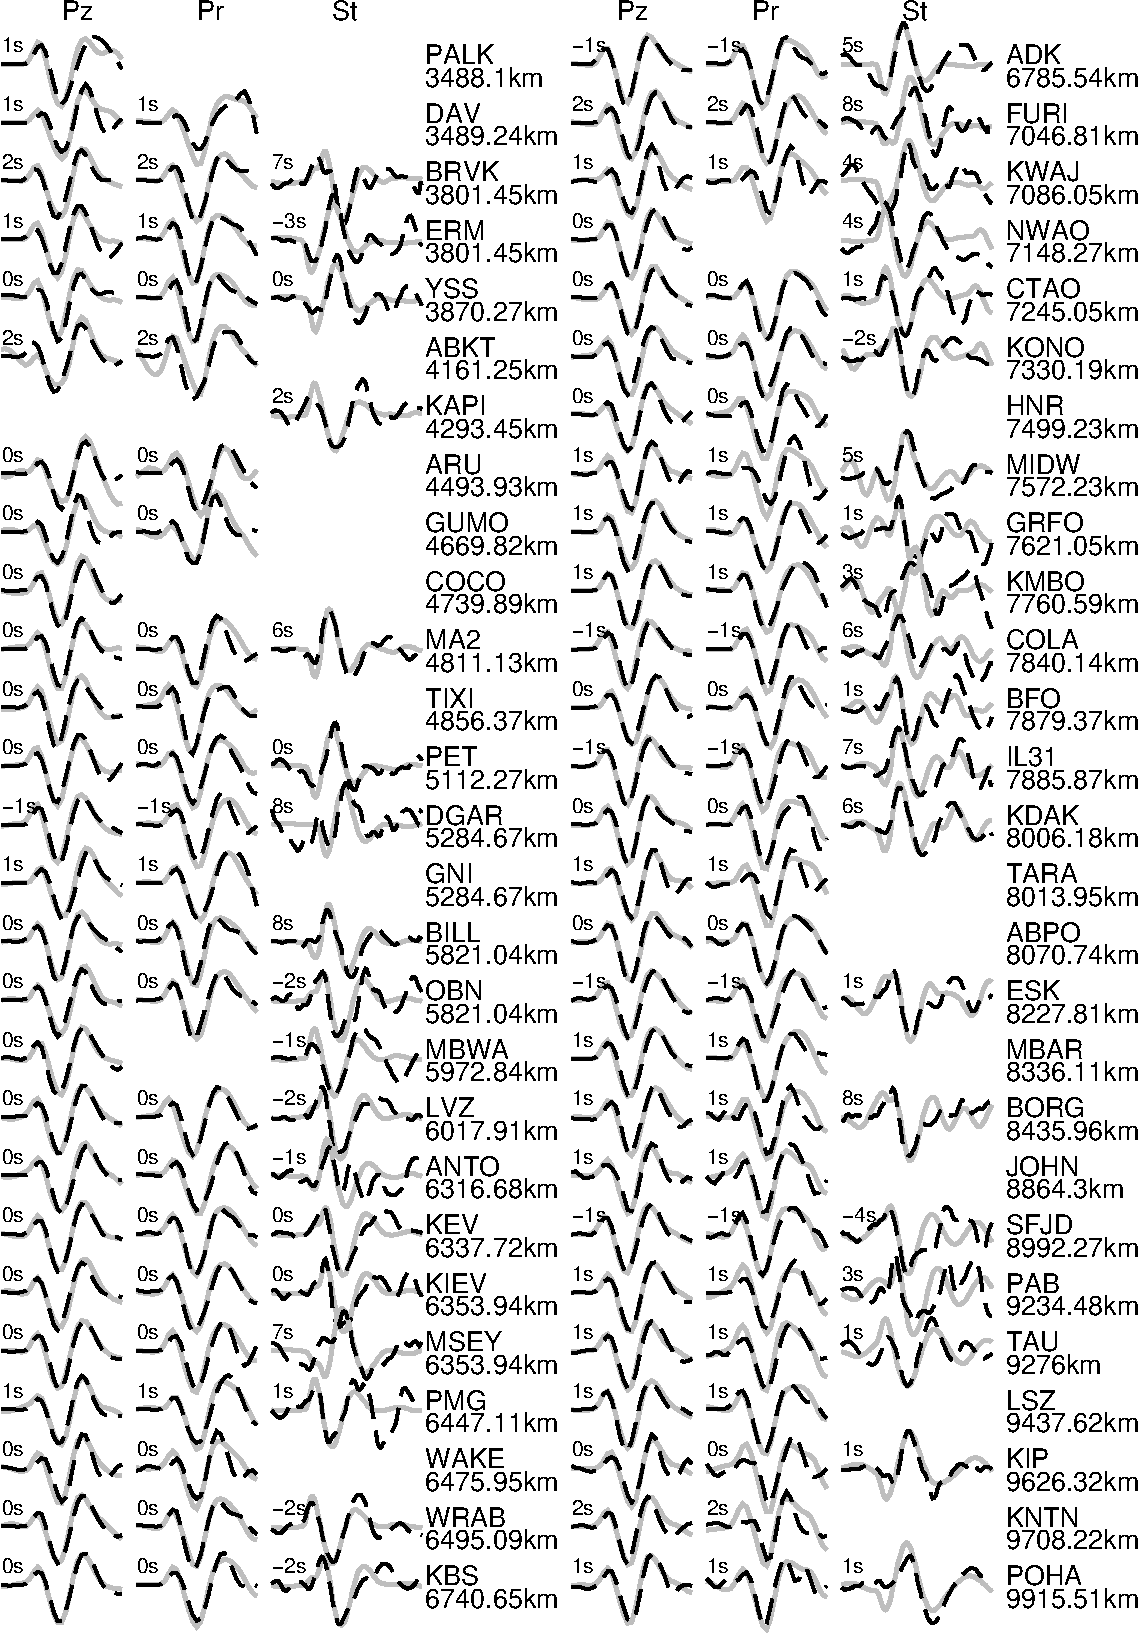
\includegraphics[scale=0.4]{fig4_04.pdf}
  \caption{ (a)(b)分别为wt(WT)加权W1加权反演各震源深度对应最佳解}
  \label{fig4_04}
\end{figure}

综上分析,W1信噪比加权通过压制高噪数据,提高反演数据的整体信噪比,能有效减弱随机噪声对反演结果的影响,增强了结果稳定性;W2振幅调节加权合理分配权重给具有振幅差异的震相波形,使反演充分利用各种震相信息,间接改善了数据结构,更好约束了反演结果,提升了结果的可靠性。

在反演时若仅考虑信噪比加权,虽然能提高结果稳定性,但是可靠性偏低,甚至出现多解情况;相反,单独考虑振幅调节加权则会降低结果稳定性。WT联合加权的效果相对更全面地考虑了结果稳定性和可靠性,在保证结果可靠性的同时,获得了较优良的稳定性,表明WT加权组的反演结果应该是三组反演组中综合效果最优的。将WT联合加权反演组的反演结果视为本文芦山地震反演的最终结果,假设误差不超过其三倍标准差大小,并结合搜索步长为1$\degree$的精度,根据\reftab{tab4_02}得到最终包含误差估计的震源机制为(走向$211\degree\pm5\degree$,倾角$41\degree\pm1\degree$,滑动角$94\degree\pm2\degree$)。

WT联合加权反演的最优震源机制所对应的所有台站理论与观测波形拟合情况如\reffig{fig4_05}所示。可以看到P波及SH波拟合得都不错,相位及其振幅均匹配得非常好。值得注意的是,同一台站的P波Z与R分量的时间平移参数非常一致,这是因为平移因子是由地震定位,发震时刻及地球速度结构等系统性误差引起的,且理论上其误差影响对于同一台站的同一震相应是相同的。此外,对于不同震中距台站的波形,拟合情况均相当,表明反演综合考虑了所有波形的信息。
\begin{figure}
\centering
  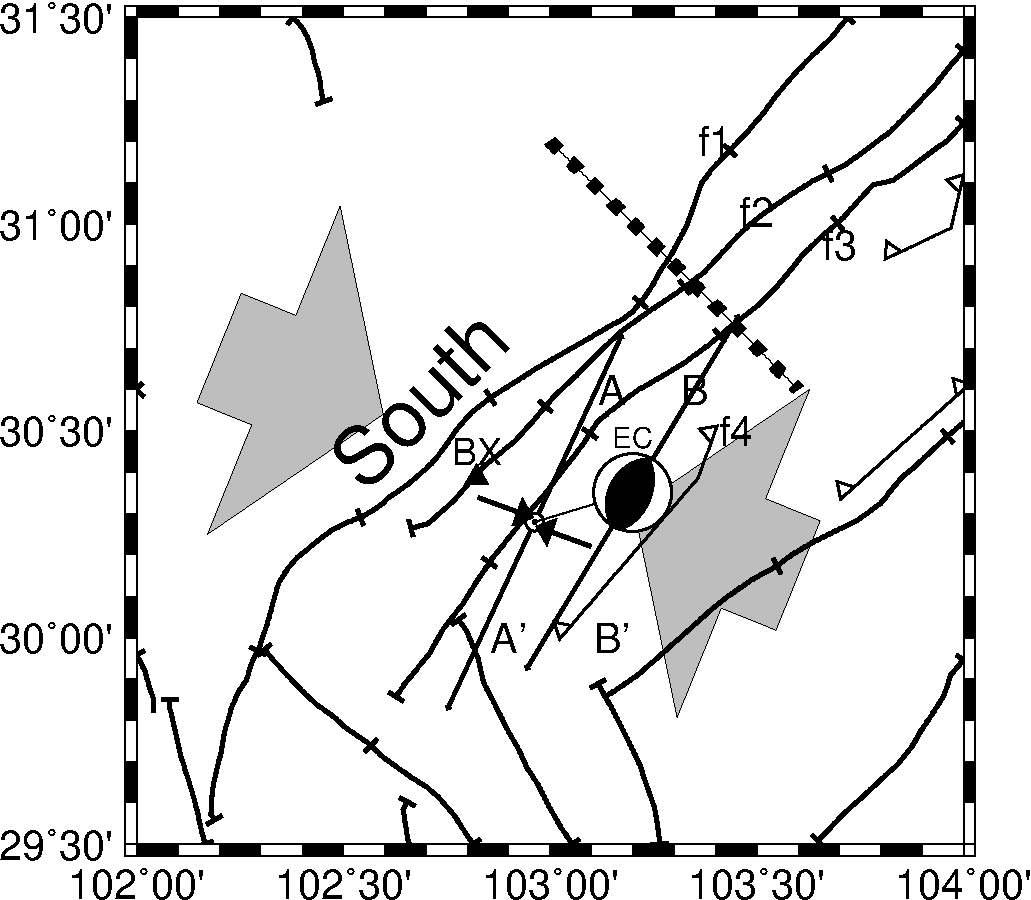
\includegraphics[scale=0.78]{fig4_05.pdf}
  \caption{ wt加权反演波形对比图,虚线为观测波形,实线为理论波形,波形右侧分别为台站名、震中距(km)。各道波形的左上方为到时差,正值表示理论到时相比实测波提前,负值相反}
  \label{fig4_05}
\end{figure}

通过本文的误差评价方法,可以得到最终震源机制的三参数间相关系数,将其列于\reftab{tab4_03}中。从之前的理论实验中,已经发现对于相同的震源机制,即使反演数据源有差异,其各参数间的相关系数仍较为相近,具有可比性。本文理论实验中所用的震源机制与反演所得的芦山地震震源机制较为相近,因此理论上其震源机制参数的相关系数也应相似。对比\reftab{tab4_03}与之前理论实验中不同噪声数据反演组对应的震源机制相关系数,可以发现芦山地震震源机制的走向和滑动角也与之前理论实验一样,体现了较强的正相关性,而倾角和另两参数的相关性相对较为不明显,基本情况近似吻合。
\begin{table}[ht]
\centering
\caption{芦山地震震源机制各参数间相关性}
\label{tab4_03}
    \begin{tabular}{c c c c}
    \hline
    相关系数 & 走向/$\degree$ & 倾角/$\degree$ & 滑动角/$\degree$ \\
    \hline
	走向/$\degree$ 		&1 			&0			&0.91\\
	倾角/$\degree$		&0			&1			&0\\
	滑动角/$\degree$	&0.91		&0			&1\\
    \hline
    \end{tabular}
\end{table}

另一方面,对于三参数中各自误差的相对大小,也可以发现,理论实验和芦山案例中震源机制倾角的误差均是最小的,走向的误差均较大。说明走向、倾角和滑动角误差的相对大小是和震源机制类型密切相关的。

芦山地震案例反演中,震源机制相关系数,和各参数误差相对大小的情况,与理论实验均有较高相似性,从侧面反映了对芦山地震估计的震源机制误差信息是较准确的。

\subsection{其它震源研究}

芦山地震后,各研究者分别对该地震震源机制进行了详细研究。\zhcitet{曾祥方}{zengxiangfang2013}利用\citet{Hardebeck2002}改进的P波初动极性反演方法及近远震波形反演方法得到了较一致的震源机制解,且借助误差曲线利用阈值类方法分析了倾角和深度的可靠性;\zhcitet{刘杰}{liujie2013}、\zhcitet{吕坚}{lujian2013}利用CAP方法对近震波形反演得到了芦山地震震源机制解,其中吕坚在波形反演基础上利用余震分布进一步约束了发震断层面;\zhcitet{谢祖军}{xiezujun2013}利用CAP方法分别对近震、远震及近远震联合反演进行对比以得到最佳震源机制。

相关研究所反演得到的震源机制均列于\reftab{tab4_04}中,可发现不同研究者所得到的结果分布情况,震源深度范围为(12km-22km),震源机制走向范围(200$\degree$-220$\degree$),倾角范围(33$\degree$-50$\degree$),滑动角范围(90$\degree$-110$\degree$),$M_w$震级(6.4-6.7)。本文反演的最终结果(震源深度17km,走向$211\degree\pm5\degree$,倾角$41\degree\pm1\degree$,滑动角$94\degree\pm2\degree$,$M_w$震级6.41)基本在此分布范围内,仅$M_w$震级略小。这一方面可能是由于本文的Fit函数的特性,为了降低系统性误差对震源机制的影响,将振幅误差归并到了震级评估中;另一方面因为各学者所用的数据及参考模型不尽相同,并且除了速度结构、地震定位以及发震时刻的不精确,理论波形的计算方法也可能导致系统性误差,相关研究表明不同程序算得的理论波形相位一致性较好,但振幅则会有一定可见差异\citep{Herrmann1985}。

\begin{table}[ht]
\newcommand{\tabincell}[2]{\begin{tabular}{@{}#1@{}}#2\end{tabular}}
\centering
\caption{不同研究者得到的芦山地震震源机制,参考自\zhcitet{吕坚}{lujian2013}}
\label{tab4_04}
    \begin{tabular}{c c c c c c c c c c c }
    \hline
    研究者 & \tabincell{c}{美国\\地调\\局} & \tabincell{c}{Global\\CMT} & \tabincell{c}{刘超\\等} &\tabincell{c}{韩立\\波等} &\tabincell{c}{中国地\\震局预\\测所} & \tabincell{c}{刘杰\\等} & \tabincell{c}{曾祥\\方等} & \tabincell{c}{谢祖\\军等} & \tabincell{c}{吕坚\\等} & \tabincell{c}{本文\\结果}\\
    \hline
	深度/km			&12	&22	&15	&12	&15	&19	&12	&16	&14	&17 \\
	走向/$\degree$	&198&210&220&220&210&214&212&210&209&211\\ 
	倾角/$\degree$	&33	&38	&35	&50	&47	&39	&47	&44	&46	&41	\\
	滑动角/$\degree$&71	&96	&95	&107&90	&100&93	&91	&94	&94	\\
	$M_w$			&6.6&6.6&6.7&6.6&6.5&6.4&6.7&6.7&6.6&6.4\\
    \hline
    \end{tabular}
\end{table}

各研究者所得的震源深度跨度较大,\zhcitet{高原}{gaoyuan2013}对地震重定位得到主震震源深度17.8km,\zhcitet{房立华}{fanglihua2013}用三维速度模型进行双差重定位给出的震源深度为17.2km和17.6km,其中房立华使用了接近震中附近的三维速度模型,并用流动观测台站对早期发生的地震进行校正,结果是较为可信的。各研究者的震源矩中心深度相对重地位的破裂点深度差异绝对值不超过5km,考虑到超过$M_w$6级的地震强度,破裂面延展可能较大,故差异相对可以接受,而本文反演的震源深度17km也是较为合理的。

\subsection{相关地质背景}
芦山地震震源位于龙门山断裂带,在该区域由于同时受到西北部青藏块体向东的挤压作用,以及东南部四川盆地坚硬地壳的阻挡,使得青藏块体东缘下方的地壳物质东流,进而导致较软弱的下地壳物质向上逆冲挤出,最终形成逆冲型的东南走向的龙门山断裂带\citep{Zhang2013}。该断裂带主要由4条大断裂构成\zhcitep{邓起东}{dengqidong1994},其整体走向为SW向\zhcitep{李智武}{lizhiwu2008}。可是从整体来看,该断裂带南北段走向具有明显的差异性\citep{Jia2006,Arne1997},\zhcitet{郭正吾}{guozhengwu1996}和\zhcitet{邓康龄}{dengkangling2007}均发现芦山地震震源区所处的南段走向相较于北段而言,有更南偏倾向。龙门山断裂带南段因受喜马拉雅期印-亚碰撞事件的重大影响,显示与松潘-甘孜褶皱带有密切关系,推断其为晚白垩世古近纪沉降中心,南段的断裂活动性延续时间较晚,直到喜马拉雅期基本定型,但现今仍在发育\zhcitep{李智武}{lizhiwu2008}。

龙门山断裂带区域的构造及地下结构一直是大家研究的热点,\citet{Zhang2013},\citet{Wang2010},\zhcitet{张忠杰}{zhangzhongjie2009}和\citet{Zhang2011}等人的研究成果表明,龙门山地区的地壳速度结构处于横向变化剧烈处,存在明显的不均匀性。根据\zhcitet{雷建设}{leijianshe2009}对龙门山断裂带地壳结构的研究,芦山地震的震源恰巧在P 波速度变化较大的区域。芦山地震震中与龙门山断裂带南段断层分布(断层数据来自\zhcitet{邓起东}{dengqidong2002})如\reffig{fig4_06}所示,由图可知震中位于南段前山断裂和山前隐伏断裂之间,地质调查结果\zhcitep{徐锡伟}{xuxiwei2013}显示芦山地震的发震断层为一条现今尚未出露地表、其上断点仍埋藏在地下地壳中的一条盲逆断层,无法直接从地表露头来观测震源断裂处走向情况,但是本文反演得到的震源机制显示的走向211°与震源区域断层整体走向基本吻合,表明反演得到的走向具有合理性。\zhcitet{唐荣昌}{tangchangrong1991},\zhcitet{李勇}{liyong2006},\citet{Densmore2007},\zhcitet{陈国光}{chenguoguang2007}等人的研究表明龙门山断裂带总体运行表现为为由北西向南东的逆冲 ,并且同时兼具有右旋走滑的特性, 整条断裂带的冲断运动由北西向南东扩展,但由于受到后山、中央、前山三条断裂带的阻碍作用,断裂带的北段和中段的山前断裂并没有明显地显现出逆冲的特征,可是芦山地震所处的南段区域却不同,其山前断裂带明显受到了冲断运动的影响,发生了较为强烈的冲断和摺皱变形,为震源所处的盲逆断层孕震提供了有利条件,与本文反演得到的滑动角所代表的逆冲型断裂发震的运动背景一致。
\begin{figure}
\centering
  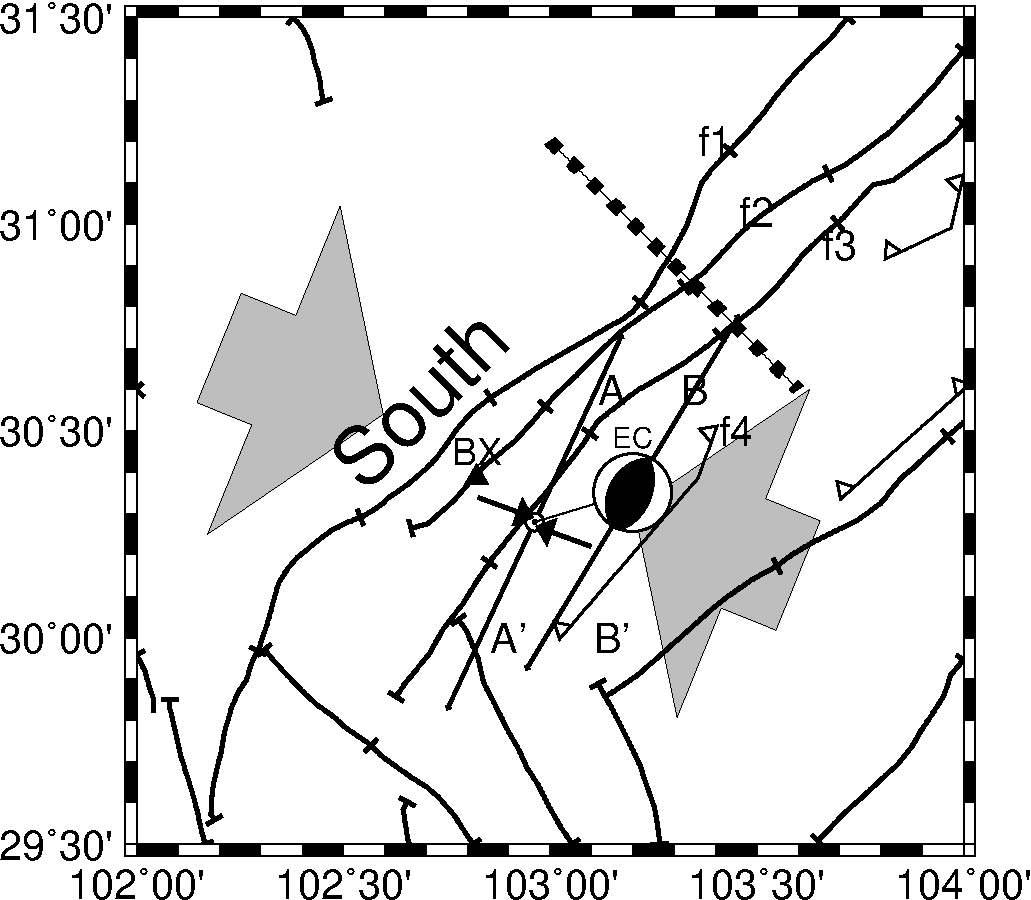
\includegraphics[scale=0.6]{fig4_06.pdf}
  \caption{ 震源区域断层与应力分布, f1,f2,f3,f4为龙门山断裂带的主要四大断裂,灰色大箭头为区域平均应力,黑色小箭头为本文震源机制对应的主压应力}
  \label{fig4_06}
\end{figure}

由于芦山地震发震断裂为盲断裂,难以直接观测发震断裂的空间构造,通过余震分布可以一定程度重现发震断裂的结构信息,\citet{zhangguangwei2013}通过双差定位发现在空间分布上主震西南方向余震分布较广、且较为集中,余震主要向西南方向扩展(\reffig{fig4_06}中AA'剖面),其剖面方向与本文震源机制的走向线BB'近乎平行,说明余震基本沿主震断层面破裂分布。

断层构造活动通常与该区域的应力分布有着密切关系,\zhcitet{孟文}{mengwen2013}实地钻孔测量研究结果表明龙门山断裂带的水平应力占主导作用,且南段的优势方向为NWW向。根据青藏高原内部存在下地壳通道流的观点\citep{Royden1997,Clark2000,Meng2005,Burchfiel1995,Harris2007},松潘-甘孜地体极有可能俯冲到四川盆地之下\zhcitep{楼海}{louhai2010},从而使得龙门山断裂带南段与青藏高原东部具有较好的连接性,是青藏高原东缘的活动边界,因此龙门山断裂带南段最大主压应力方向与区域应力场方向一致,为NW-NWW向,孟文等的钻井数据显示距震中较近的宝兴钻井点主应力方向为N80°W至N74°W,另一钻井结果表明宝兴主应力方向为N60°W\zhcitep{秦向辉}{qinxianghui2013},上述区域应力方向以及实际钻井没得的主应力方向均与本文反演所得的震源机制主应力方向一致。

研究表明, 快剪切波偏振的优势方向一般与原地主压应力方向一致\citep{Gao2011,Gao2012},\zhcitet{高原}{gaoyuan2013}用剪切波分裂的方法计算发现位于芦山地震震中东北方向的龙门山断裂带中南段的台站快剪切波偏振的优势方向近似为NW 向,与断裂带走向近似垂直;而在芦山地震震中西南方向的龙门山断裂带南段靠近鲜水河断裂处,快剪切波偏振方向表现得比较离散,但平均方向为近EW方向,所以地理位置位于其中间的震中区的偏振优势方向极有可能在NW与EW之间。此外\zhcitet{赵博}{zhaobo2013}利用力轴张量法计算得到的芦山地震余震分布区的平均压应力方向约为112°,如\reffig{fig4_06}中灰色大箭头所示。本文震源机制(走向211°,倾角41°,滑动角94°)对应的P轴近水平,与各向异性分析及力轴张量计算法得到的应力结果有很好的一致性。上述钻井实测资料,应力计算资料结果相互吻合,均与本文震源机制表现出一致性,表明芦山地震主要为区域NWW向水平应力长年积累的一次应力释放。

\section{结论}
芦山地震实例反演中,震源机制误差大小与不同加权稳定性的预测一致,且该案例中三参数误差的相对大小和它们之间的相关性,与相近地震类型的理论事件情况相似,均表明对芦山地震震源机制的误差估计较可靠,证明了本文误差估计方法在真实地震案例中的实用性。

根据不同加权的三组反演对照组的对比结果,W1信噪比加权抑制了噪声干扰,明显提高了拟合度,并且减小了结果误差,增强了稳定性。W2振幅调节加权合理为振幅不同的震相分配权重,间接优化了数据结构,防止了33km震源深度附近极值点的出现,减弱了结果的多解性,增强了结果的可靠性。WT联合反演吸收了W1和W2的优点,全面考虑了数据信噪比和数据结构,综合提升了结果的稳定性和可靠性。

本文反演芦山地震的最终结果——震源深度17km,震源机制(走向$211\degree\pm5\degree$,倾角$41\degree\pm1\degree$,滑动角$94\degree\pm2\degree$),与其它研究者的结果有良好一致性,且与震源区域的地质构造背景和应力情况相符合,表明本文反演结果较为可信。根据应力分布、地震定位及构造情况,推断本次地震震源为由区域水平向应力长期积累下的势能释放,导致的高倾角近纯逆冲型滑动断裂。
 %第四章 实例应用
%------------------------------------------

\chapter{总结和展望}
\section{主要创新点}
本文最主要的创新性工作是提出了一种评估震源机制误差信息的方法。鉴于目前国内外利用地震波反演震源机制时,普遍缺少误差评定的现状,并考虑到误差评定对科学研究的重要意义,针对利用地震波拟合反演震源机制中应用较广泛的格点搜索法程序——CPS和CAP,探讨了给予反演误差的思路。首先根据误差信息的相关理论,从其定义出发严谨推导,并得到了相应的理论基础。进而大胆提出了适用于震源机制反演的误差评价方法,评估其可行性并快速实现了方法所需程序。其后慎重考虑了执行中的可能变数,通过理论实验严格检验了该方法的成效。
相比\citet{zhenjianchang2015}随机重采样的误差统计方法,本文方法没有改变原始数据分布,并且保留了所有可用观测数据,因此理论上对观测数据总量要求相对较宽松,适用范围更广。

另一项主要工作是基于CPS和CAP的加权方案,通过权重精化和联合进行了优化。针对CPS和CAP的加权计算方法,比较之下发现其计算的权重数值相对大小存在的矛盾点。随后,考虑了各自加权的主要原因,并深入探讨各方案加权的本质以及对反演的影响,从理论上分析了权重联合的可能性以及预期优化效果。之后对联合加权和单独加权方案进行对比检验,分别从理论实验和实例反演两方面进行了对照组反演,结合结果评价了联合定权的优势。

\section{工作总结}
理论实验和实例应用中对误差的估计和讨论,充分说明了本文所提出针对震源机制误差评价方法的有效性,其准确反映了数据随机噪声的存在对于反演得到的震源机制的影响,明确给出了误差范围。并且还揭示了震源机制各参数间的相关性,对于进一步推测误差的情况起到了一定指导作用。在理论实验中,对于高信噪比数据反演参照组,发现即使在数据噪声含量比较低的情况下,误差仍然不可忽略,证明了在实际工作中反演震源机制时评估数据随机噪声影响的重要性和必要性,肯定了本文工作的意义。
事实上,由于本文误差估计方法基于误差定义的理论基础,因此不仅限于格点搜索反演,也不仅针对震源机制反演,对所有已知数据噪声信息,但未能评价结果误差的反演问题均是一种可行方案。

权重优化的对比实验表明了本文联合加权方案在一定程度上对反演结果进行了优化。但是需要注意,对反演结果有根本决定作用的是原始观测数据质量,包括数据信噪比和数据结构。数据信噪比表征了数据信息的真实程度,因为随机噪声相当于虚假信号,对结果具有干扰作用。数据结构则表征了数据信息总量的约束强度,即使数据没有任何误差,当结构分布很差,数据不足时也无法得到唯一真实解,这相当于欠定反演问题。只有当数据质量达到反演满足的最低要求时,合理地加权才能显示出优化结果的作用。本文联合加权中的信噪比权重W1针对数据信噪比,降低了低信噪比数据的影响,并最终提高了代表反演结果稳定性的拟合度。而振幅调节权重W2则是从数据结构着手,通过合理平衡不同数据在反演中的影响力,相当于间接“增加”了参与反演的数据数量,增强了反演的约束力度,使结果更可靠。

对芦山地震的反演展示了本文误差估计方法的实用性以及权重优化在实际工作中的效果,对本文震源机制(走向$211\degree\pm5\degree$,倾角$41\degree\pm1\degree$,滑动角$94\degree\pm2\degree$)和他人成果的对比分析表明,余震基本沿主震断层面破裂分布,延展趋势与本文走向匹配;芦山地震所处的南段区域,其山前断裂带明显受到了冲断运动的影响,发生了较为强烈的冲断和摺皱变形,为震源所处的盲逆断层孕震提供了有利条件,与本文所得到的逆冲型断裂发震的运动背景一致;震源区钻井实测资料,快剪切波应力计算资料结果相互吻合,均与本文震源机制的滑动角、倾角所暗示的应力情况表现出一致性,表明芦山地震主要为区域NWW向水平应力长年积累的一次应力释放。

通过多次实验结果对比,以及相关理论公式,推测震源机制各参数的误差绝对大小不仅与原始观测数据噪声相关,还和具体的震源机制类型有密切联系。相比之下,各参数误差的相对大小、以及各参数间的两两相关性则主要和地震的震源机制相关,观测数据的噪声对其影响很小。

\section{展望}
本文最核心的工作是针对震源机制反演过程中误差评定缺失问题,给出了一个解决方案——通过模拟噪声和数据进行重复反演,并利用统计手段估计得到误差信息。虽然该方法经过推导、理论实验均证明可靠有效,但是仍然有许多不足及有待改进的地方。

首先,本文明确指出所研究的误差信息仅包括来源于观测数据随机噪声的部分,这并不是表示其它诸如地下速度结构偏差导致的系统性误差在震源研究中不重要。恰巧相反,本文的相关实验暗示了系统性误差的影响不权并非微不足道,而且可能比随机噪声的影响还大。因为基于本文的误差估计,发现在理论实验和真实反演案例中,即使原始数据的噪声强度相近,理论实验的数据拟合度仍显著高于实际地震反演的拟合度。这说明其中还有除数据噪声以外不可忽视的干扰,合理推断应该是来源于真实地下结构与参考模型的差异、以及对真实地震过程进行模型简化后的影响。

从理论上分析,本文的误差估计方法基于数据噪声的随机分布,利用噪声期望与分布的特点,通过重复试验统计分析随机噪声的影响。然而系统性误差不具备这样的特性,无法通过多次重复反演进行消除或评估其影响。因此,从原理上讲,本方法不适用于对系统性误差的研究。如果强行尝试,一种考虑方案是利用随机噪声的方式对待系统性误差,将其随机化,如将参考模型像数据噪声一样给出一定的误差范围,并在反演中考虑其可能偏差的影响。但是每次模型的不同偏差必然需要重新计算格林函数库,格林函数库计算是震源机制反演中最耗时的步骤,这在重复的大量反演中将带来不可接受的计算量,因此不具备实际可行性。因此对系统误差的考虑,仍旧需要进一步研究,寻找其它解决方案。

介于以上原因,在本文工作中由于模型偏差等系统性偏差的研究欠缺,便直接忽略了系统误差,事实上该误差的影响有可能比随机误差更大,值得在之后的研究中关注。

其次,对误差统计分析的关键在于制造解的随机集合,尽可能使误差估计接近真实情况。从概率统计角度考虑,这要求进行大量的重复反演,才能保证误差范围具有相对较高的可信度。但是大量的重复反演,直接倍增了总的计算时间,降低了反演效率。因此本文的误差估计方法不适合应用于对实时性要求较高的自动化系统中,而是相对更适合于对速度要求相对宽松的后期精化研究中。

考虑到上述本文误差评价方法的两点不足,除了进一步优化本文方法,另一种可选方案是直接从其它思路考虑。如\citet{Duputel2012}关注了震源机制反演过程中普遍缺少误差评价的问题,意识到误差估计的重要性,并就此较为系统地讨论了震源机制反演中的各种误差。不过他的研究是基于另一种较新颖的线性化的震源机制反演方法,解决方案对于国内应用更普遍的CAP类搜索方法并不适用。不过以后更多的反演方法可能被广泛接受,因此更完备的误差评价方法也可能受到更多关注。因此从根本的反演算法角度考虑,解决误差评价问题也值得将来进一步思考。
 %第五章 总结和展望
%---参考文献------
\cleardoublepage
\phantomsection
\addcontentsline{toc}{chapter}{参考文献}   
\bibliography{BIBbase/ref}%参考文献
%---------------------------------------
%\include{includefile/pub}
%-----------------------------------------
\backmatter
% !Mode:: "TeX:UTF-8"

%%% 此部分内容:  (1) 致谢  (2) 武汉大学学位论文使用授权协议书(无需改动)

%%%%%%%%%%%%%%%%%%%%%%%
%%% --------------- 致谢 ------------- - %%%
%%%%%%%%%%%%%%%%%%%%%%%
\acknowledgement

历经多年,一步步走到硕士研究生,并至现在完成硕士毕业论文,我最想感谢的是我的家人。这一切离不开父母和其它家人的支持和无私付出。我的父母并没有受过太多教育,我也一家人中唯一进入过大学校园学习的。从小,父母便对我的教育格外重视,虽然为了家里孩子的生计,长年在外奔波,一年到头只有过年才能相聚,但每次打电话必然会考察我的学习情况。虽然随着所受教育越来越高,父母已经不能完全明白大学已来的教育方式和主旨,但在学习上我所需要的,他们从来没有质疑或犹豫,一直尽他们所有默默支持着我的选择。姐姐和兄长在出去工作后,也用自己的辛劳帮助渐渐年迈的父母,支持起这个家,资助我的学业。在此,对他们的无私付出由内心表示感谢,也会鞭策自己继续努力,不负他们的期望。

在整个研究生生涯,导师承担了老师和长辈的负责。一方面,用他在理论方面的造诣对我的研究和疑惑进行指导,对导师在地震学理论方面的知识背景由衷佩服,其课程和讨论对我的毕业课题研究带来了灵感。另一方面,他作为长辈,在生活中,对我体现了莫大关怀、包容。在研究生期间遇到挫折时,他没有给我压力,反而是给了我足够的时间和理解。让我得以重新恢复、振作。在此,由衷感谢

我研究生所在的师们,师兄弟不算很多,但是我们很团结。师兄们就像兄长一样,对我进行指引,给予我帮助。当然,还少不了各种各样的聚餐和活动。大师兄王清东为人和善,对所有问题都非常乐观。陈浩朋做事细致,努力,常常帮我仔细地修改论文问题至一句一词。杨颖航在读硕期间连发两篇高质量文章,是优秀的榜样。张攀在我的研究中提供了不少帮助,这篇毕业设计的LATEX版就是在他帮助下完成的。王光明和我从大学起就是同学,常常能够和我讨论一些生活,学习中的问题,在我颓废时给了我很大的鼓励。黄杰基础好,求知心强,能给出不错的见解和建议。

最后,要感谢在本文工作中所使用的CPS、Taup和GMT绘图软件的作者,将这样优秀软件无私提供给他人使用。尤其特别感谢Doc. Herrmann对本文反演研究给予中给予的相关指导和解惑。反演数据来自IRIS,在此一并感谢。




%%%%%---武汉大学学位论文使用授权协议书---%%%%%%%%%%%%
%%%%%%%%%%%%%%%%%%%%%%%%%%%%%%%%%%%
%%%%%%%%%%%%%%%%%%%%%%%%%%%%%%%%%%%
\cleardoublepage
\newpage\vspace*{20pt}
\begin{center}{\zihao{-2}\heiti 武汉大学学位论文使用授权协议书}\end{center}
\par\vspace*{30pt}

本学位论文作者愿意遵守武汉大学关于保存、使用学位论文的管理办法及规定,
即:学校有权保存学位论文的印刷本和电子版, 并提供文献检索与阅览服务;
学校可以采用影印、缩印、数字化或其它复制手段保存论文;
在以教学与科研服务为目的前提下, 学校可以在校园网内公布部分及全部内容.
\begin{enumerate}[1、]
  \item  在本论文提交当年, 同意在校园网内以及中国高等教育文献保障系
           统(CALIS)高校学位论文系统提供查询及前十六页浏览服务.
  \item  在本论文提交~$\Box$~当年/~$\Box$~一年/~$\Box$~两年
            /~$\Box$~三年/~$\Box$~五年以后, 同意在校园网内允许读者
            在线浏览并下载全文, 学校可以为存在馆际合作关系的兄弟高校用
            户提供文献传递服务和交换服务.(保密论文解密后遵守此规定)
\end{enumerate}

\vskip 15mm

论文作者(签名):\raisebox{-1ex}{\underline{\makebox[5cm][c]{}}}
\vskip2em
				          				
学\qquad\qquad\quad 号:\raisebox{-1ex}{\underline{\makebox[5cm][c]{}}}
\vskip2em	
					
学\qquad\qquad\quad 院:\raisebox{-1ex}{\underline{\makebox[5cm][c]{}}}					

\vskip  2cm
\begin{flushright}
 日期:\hskip2cm 年\hskip1.2cm 月\hskip1.2cm 日
\end{flushright}

%%%%%%%%%%%%%%%%%%%%%%%%%%%%%%%%%%%%%%%
%%%%%%%--判断是否需要空白页-----------------------------
  \iflib
  \else
  \newpage
  \cleardoublepage
  \fi
%%%%%%%-------------------------------------------------








\cleardoublepage
\end{document}
